\documentclass[a4paper,11pt,oneside,roman]{article}
\usepackage{multirow}

\usepackage{ifxetex}
\ifxetex
\usepackage{fontspec}
\else
\usepackage[utf8]{inputenc}
\usepackage{lmodern}
\usepackage{textcomp}
\usepackage[T1]{fontenc}
\usepackage[top=2cm, left=2cm, right=2cm, bottom=2cm]{geometry}
\usepackage[francais]{babel}
\fi
\usepackage{color}
\usepackage{amsmath}
\usepackage{graphicx}
\usepackage{amssymb}
\usepackage{stmaryrd}
\usepackage{listings}
\usepackage{parskip}
\usepackage{float}
\floatplacement{figure}{H}
\lstset{language=C,
 %
    inputencoding=utf8,
    extendedchars=true,
    literate=%
            {é}{{\'{e}}}1
            {è}{{\`{e}}}1
            {ê}{{\^{e}}}1
            {ë}{{\¨{e}}}1
            {û}{{\^{u}}}1
            {ù}{{\`{u}}}1
            {â}{{\^{a}}}1
            {à}{{\`{a}}}1
            {î}{{\^{i}}}1
            {ô}{{\^{o}}}1
            {ç}{{\c{c}}}1
            {Ç}{{\c{C}}}1
            {É}{{\'{E}}}1
            {Ê}{{\^{E}}}1
            {À}{{\`{A}}}1
            {Â}{{\^{A}}}1
            {Î}{{\^{I}}}1,
	aboveskip=3mm,
	belowskip=3mm,
	numbers=left,
	keywordstyle=\color{blue},
	commentstyle=\color{dkgreen},
	breaklines=true,
	breakatwhitespace=true,
	tabsize=4,
	frame=single
}
\lstset{showstringspaces=false}
\usepackage{hyperref}

\title{SY09 - Compte Rendu de Projet 2}
\author{LIBRAIRE Audrick - NGUYEN Anh Tu}
\date{\today}

\begin{document}
\maketitle

\tableofcontents \newpage
\section{Introduction}
Pour ce deuxième rendu de projet de l’UV SY09, nous avons appliqué plusieurs méthodes vues en cours, qui concernent la discrimination et la régression. La discrimination est pour l’objectif d’apprendre un modèle qui permettra de déterminer la classe à partir des observations des variables explicatives pour de nouveaux individus alors que la régression nous permet de lier les variables observées à la variable à expliquer pour déduire la valeur d'une variable quantitative. Dans le cadre de ce projet, nous avons effectué des analyses pour évaluer les performances des principales méthodes de discrimination étudiées dans le cours : analyse discriminante quadratique et linaire, classifieur bayésien naïf, regression logistique et arbre de décision sur des différents jeux de données en utilisant des fonctions effectuées dans TDs et des fonctions du biliothèque \textbf{MASS} de R. 

\section{Discrimination}
\subsection{Breastcancer}
\subsubsection{Analyse exploratoire}
Tout d'abord, nous avons effectué une analyse exploratoire pour comprendre et s'approcher les données fournies. \newline
Ce jeu de données comporte 30 variables et 569 individus. On a exclu la premère colonne parce que cela correspond à l'index qui est inutile dans notre analyse. Nous avons puis obtenu le jeu de données à analyser.\newline
\begin{figure}[h]
    \centering
    \begin{tabular}{cc}
    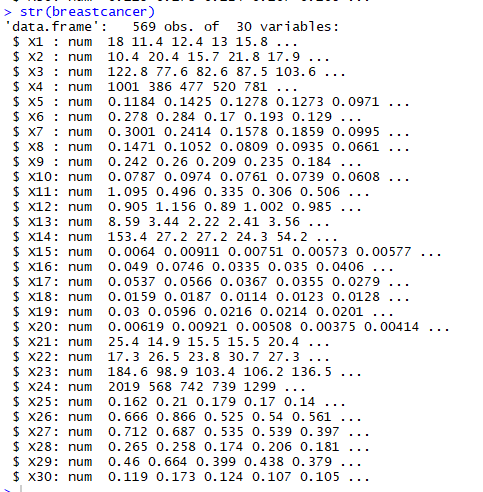
\includegraphics[scale = .6]{./discrimination/breastcancer/structure.PNG} \\
    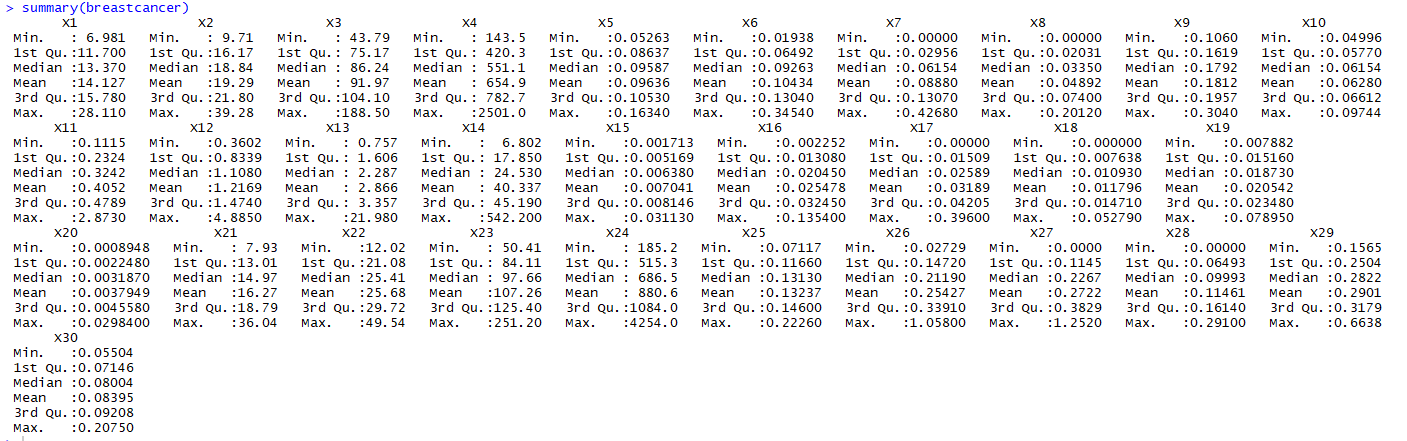
\includegraphics[scale = .5]{discrimination/breastcancer/summary.PNG}
    \end{tabular}
    \caption{La structure du jeu de données \textbf{breastcancer}}
    \label{fig:my_label}
\end{figure}
A partir des résultats ci-dessus, on peut voir que toutes les variables sont des variables numériques. Plupart de variables sont compris entre $0$ et $1$, il y a quelques variables ayant les valeurs qui sont beaucoup plus grandes que les autres par exemple $X4$, $X24$. D'autre part, dans le but d'étudier la corrélation entre les variables qui peut produire des influences dans les méthodes de discrimination, nous avons un graphique chacun des variables. \newline
\begin{figure}[htb]
    \centering
    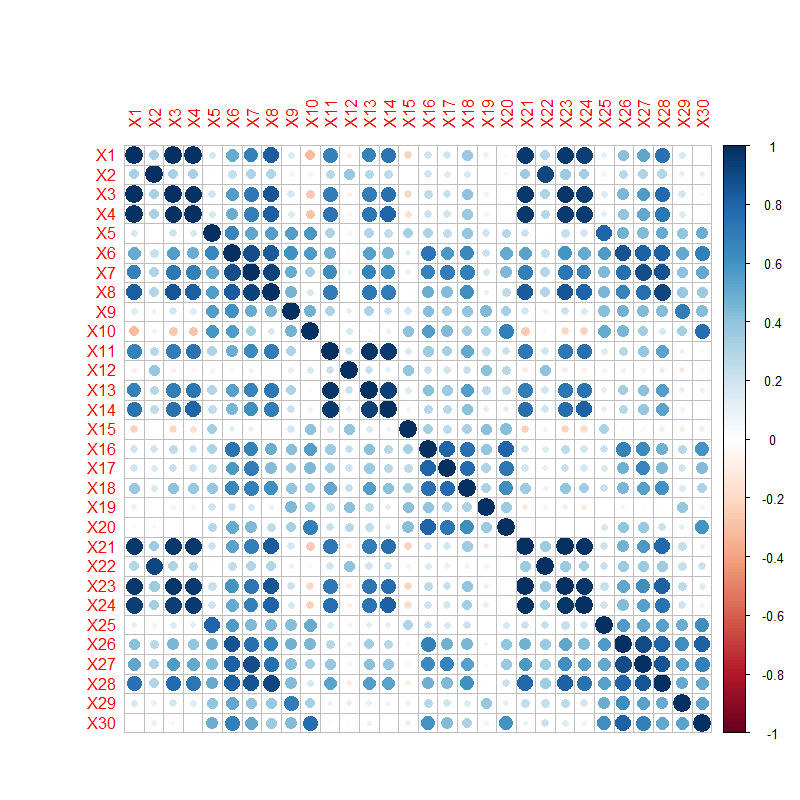
\includegraphics[scale = .4]{./discrimination/breastcancer/correlation.png} 
    \caption{La corrélation entre les variables de \textbf{breastcancer}}
    \label{fig:my_label}
\end{figure}
Le test de corrélations a été réalisé par la méthode de Pearson avec \textbf{p-value} a été fixée par défault pour $\alpha = 0.05$. Grâce au graphique, on peut observer facilement qu'il y a des paires très corrélé  comme $(X1,X3)$, $(X1,X4)$, $(X21,X3)$. L'étude de la corrélation est poursuivie par la réalisation d'analyse en composantes principales. Nous avons décidé de réaliser l'analyse en composante principales parce que on veut au premier temps explorer la géométrie des données et à partir de cela, on peut prévoir le modèle compatible. 
L'analyse en composantes principales \(ACP\) est un outil permettant d'annalyser et visualiser un jeu de données contenant des individus décrits par plusieurs variables. L'ACP nous donne une première vue et une première idée de la géométrie de nos données. Nous avons obtenu d'abord 2 graphiques : le cercle de corrélation et l'inertie de valeurs propres de 10 premières valeurs en utilisant la fonction \textit{princomp} et des fonctions du biliothèque \textit{factoextra}.
\begin{figure}[htb]
    \centering
    \begin{tabular}{c|c}
    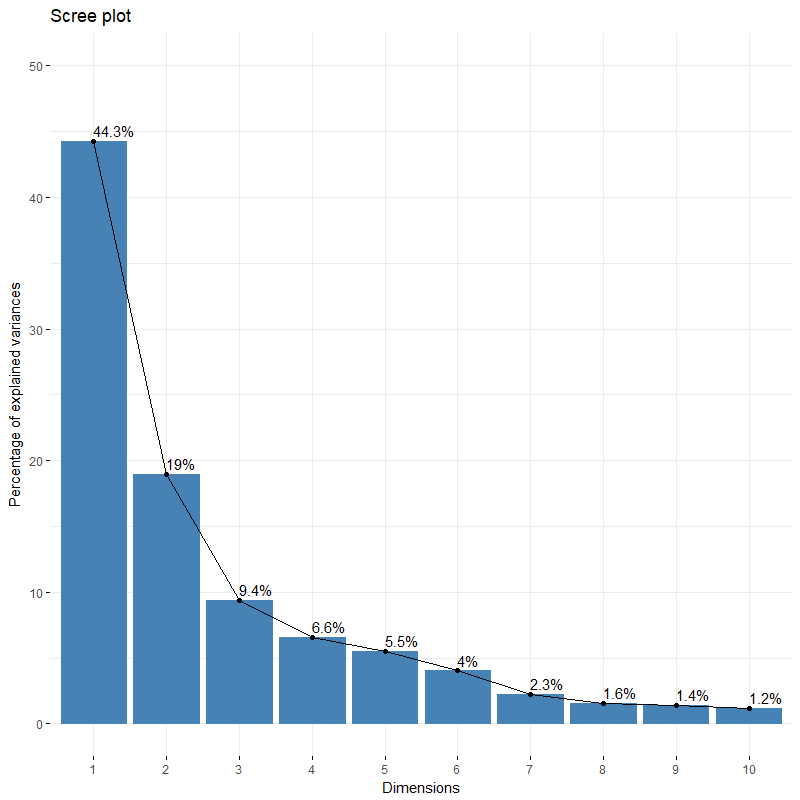
\includegraphics[scale = .3]{./discrimination/breastcancer/eig.png} &
    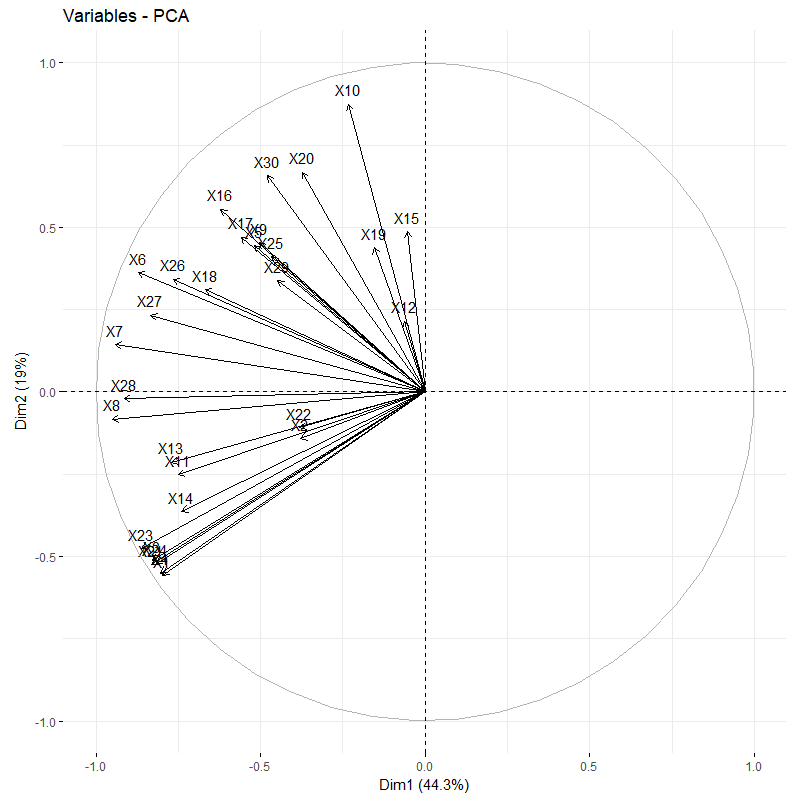
\includegraphics[scale = .3]{discrimination/breastcancer/variables.png}
    \end{tabular}
    \caption{Graphique a : L'inertie de valeurs propres de 10 premières valeurs - Graphique b : Le cercle de corrélation des variables \textbf{breastcancer}}
    \label{fig:my_label}
\end{figure}
Dans le cadre de notre analyse, nous pouvons voir que les informations se concentrent aux 7 premières composantes avec plus de 90\% des informations totales. De plus, le cercle de corrélation des variables expliqué par les deux premières composantes nous montre la corrélation entre les variables. On peut vois dans le cercle de corrélation que toutes les variables ont tendance l'inverse au sens de la deuxième composantes et cela est intéressante si on observe la distribution des individus dans le graphique des individus ci-dessous : 
\begin{figure}[htb]
    \centering
    \begin{tabular}{cc}
    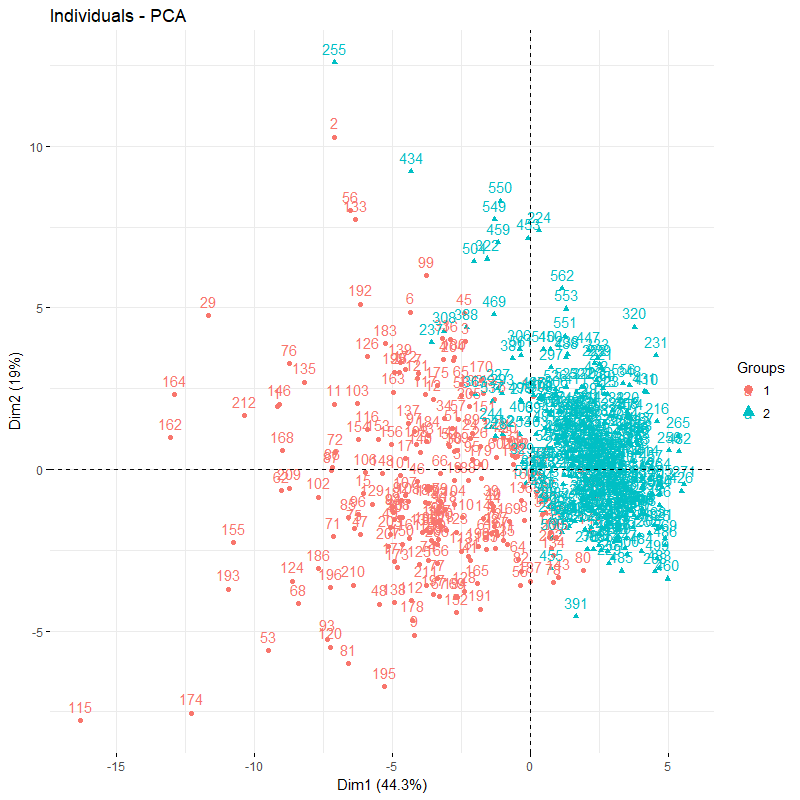
\includegraphics[scale = .4]{./discrimination/breastcancer/indi_plot12.png} &
    \end{tabular}
    \caption{La distribution des individus dans 2 premières composantes \textbf{breastcancer}}
    \label{fig:my_label}
\end{figure}
La distribution des individus dans le graphique est très claire : les individus de classe 1 sont distribuées à la gauche de l'axe $y=0$ et sont distribuées selon les variables (les individus se situent très proche des vecteurs des variables) tandis que les individus de classe 2 se situent à gauche de l'axe $=0$ et ont tendance plus concentrée selon l'axe $x=0$. Les deux classes sont séparées assez clairement donc nous pouvons prévoir que l'analyse de discriminante linéaire peut nous donner une bonne classification. Pour vérifier notre prédiction, nous viendrons la réalisation des méthodes de discrimination sur ce jeu de données.
\subsubsection{Réalisation des méthode de discrimination}
Pour calculer le taux d'erreur ponctuelle $\Hat{\epsilon}$ d'une prédiction, il faut simplement compter le nombre de prédiction erronées $\epsilon_i$ entre la prédiction faite et les données réelle (d'apprentissage ou de test), puis diviser par le nombre total d'individus \textit{n}. \newline
On répète cette procédure 100 fois pour obtenir 100 réalisations du taux d'erreur. Pour obtenir l'estimation du taux d'erreur $\Bar{\epsilon}$, il ne reste plus qu'à faire la moyenne des 100 réalisations. \newline
L'intervalle de confiance à 95\% est obtenu comme-ci : $IC = \left[\mu - 1.96*\frac{s^{*}}{\sqrt{N}};\mu + 1.96*\frac{s^{*}}{\sqrt{N}} \right]$ avec : \newline
\begin{itemize}
    \item $\mu$ : La moyenne des 100 réalisation de $\epsilon$ \\
    \item $s^{*}$ : L'écart-type corrigé des 100 réalisations de $\epsilon$ \\
    \item $N$ : Le nombre de réalisation et dans ce cas $N=100$
\end{itemize}
Nous avons appliqué des différents modèles d'analyses discriminantes, de régression logistique ainsi que les arbres de décisions. Le résume des résultats sont en table ci-dessous.
\begin{table}[H]
\centering

\begin{tabular}{l|l|cc}
\multicolumn{1}{l|}{\textbf{Méthode}}    & \textbf{Données} &$ \overline{\varepsilon}$ & $IC$                      \\ \hline
\multirow{2}{*}{Analyse discriminante quadratique} & Apprentissage    & 0.6104                   & $\left[0.6092 ;~ 0.6118 \right]$  \\
                                       & Test             & 0.6109             & $\left[0.6093  ;~ 0.6126 \right]$ \\ \hline
\multirow{2}{*}{Analyse discriminante linéaire}                  & Apprentissage & 0.0800                                 & $\left[0.0785 ;~ 0.0816 \right]$  \\
                                       & Test             & 0.0884                       & $\left[0.0846  ;~ 0.0921 \right]$ \\ \hline
\multirow{2}{*}{Classifieur bayésien naïf}                  & Apprentissage    & 0.3702                             & $\left[0.3699 ;~ 0.3704 \right]$  \\
                                       & Test             & 0.3722                                 & $\left[0.3717 ;~ 0.3726 \right]$ \\ \hline
\multirow{2}{*}{Régression logistique (intercept=1)}                  & Apprentissage    & 0.0327                             & $\left[0.0235 ;~ 0.0419 \right]$  \\
                                       & Test             & 0.0325                                 & $\left[0.0183;~ 0.0466 \right]$ \\ \hline
\multirow{2}{*}{Régression logistique (intercept=0)}                  & Apprentissage    & 0.0321                           & $\left[0.0284 ;~ 0.0360 \right]$  \\
                                       & Test             & 0.0426                                & $\left[0.0337 ;~ 0.0515 \right]$ \\ \hline
\multirow{2}{*}{Régression logistique quadratique (intercept=0)}                  & Apprentissage    &  0.0322                            & $\left[0.0203 ;~ 0.0420 \right]$  \\
                                       & Test             & 0.0356                                & $\left[0.0215;~ 0.0497 \right]$ \\ \hline
\multirow{2}{*}{Régression logistique quadratique (intercept=1)}                  & Apprentissage    & 0.0282                            & $\left[0.0232 ;~ 0.0331\right]$  \\
                                       & Test             & 0.0405                                 & $\left[0.0308 ;~ 0.0502 \right]$ \\ \hline      
\multirow{2}{*}{Arbre de décision}                  & Apprentissage    & 0.0393                             & $\left[0.0351 ;~  0.0436 \right]$  \\
                                       & Test             & 0.0726                                 & $\left[0.0654 ;~ 0.0798 \right]$ 
\end{tabular}

\caption{Calcul du taux d'erreur d'apprentissage $\varepsilon$ et de test pour le jeu de données breastcancer avec plusieurs méthodes (arrondi à $10^{-4})$}
\label{breastcancer}
\end{table}
On remarque ici que dans le cas de la régression logistique, on ne peut pas réaliser l'analyse sur le jeu de données initial car dans certains cas nous obtenons ce résultat : $det(X^{T}W_{q}X) =  0$ donc il n'est pas possible d'inverser cette matrice. On crois que dans ce jeu de données, il y trop de paramètres à estimer, notamment dans le cas de régression logistique quadratique mais on n'a que 569 individus et après avoir séparé en ensemble d'apprentissage et ensemble de test, il n'y a que 379 individus pour l'apprentissage. Nous donc décidons d'utiliser l'ACP avec le fait que l'informations se concentrent aux 7 premières composantes avec plus de 90\%. \newline
\begin{figure}[htb]
    \centering
    \begin{tabular}{cc}
    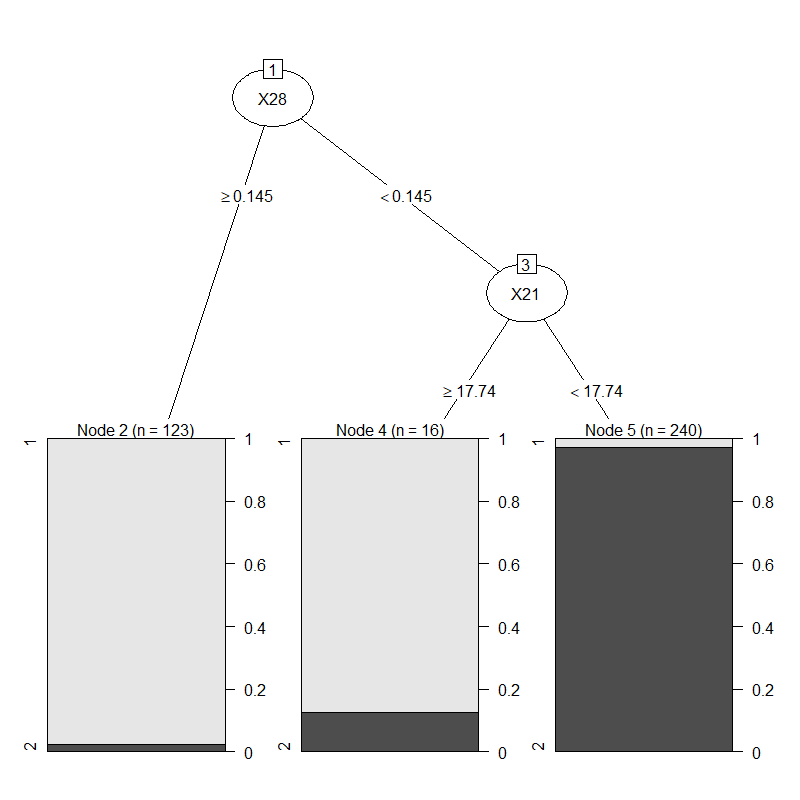
\includegraphics[scale = .4]{./discrimination/breastcancer/tree.png} &
    \end{tabular}
    \caption{L'arbre de décision \textbf{breastcancer}}
    \label{fig:my_label}
\end{figure}
\newline
D'après la table \ref{breastcancer}, la régression logistique permet d'obtenir les très bonnes résultats après le traitement de données par l'ACP. Comme nous choisissons les composantes qui conservent plupart d'informations, le nombre de paramètres à estimer de la régression logistique est moins que les autres méthodes. Deplus, la régression logistique est plus robuste et flexible que les autres, notamment dans le cas où les individus ne sont pas distribués normalement. C'est pourquoi on peut obtenir des très bons résultats avec la régression logistique sans perdre beaucoup de l'informations en utilisant ACP. Le résultat obtenu par l'arbre de décision est rémarquable. L'arbre de décision est une méthode interprétable mêmi si dans le cas de grande dimension. Comme nous avons prévu, l'analyse discriminante linéaire peut nous donner un bon résultat. Le classifieur bayésien naïf et l'analyse discriminante quadratique déduit des mauvais résultats notamment l'analyse discriminante quadratique. Le classifieur bayésien naïf est trop simple pour exprimer les données \textbf{breastcancer} tandis que l'analyse discriminante quadratique est trop compliquée. Nous avons essayé l'analyse discriminante quadratique avec des données traitées par l'ACP comme le cas de la régressions logistique et nous avons obtenu 0.0712 pour le taux d'erreur d'apprentissage et 0.0506 pour le taux d'erreur de test. 

\subsection{Ionosphere}
\subsubsection{Analyse exploratoire}
Comme le jeu de données précédent, nous avons d'abord effectué une analyse exploratoire pour comprendre et s'approcher les données fournies. \newline
Ce jeu de données comporte 34 variables et 350 individus. On a exclu la première colonne parce que cela correspond à l'index qui est inutile dans notre analyse.
\begin{figure}[htb]
    \centering
    \begin{tabular}{cc}
    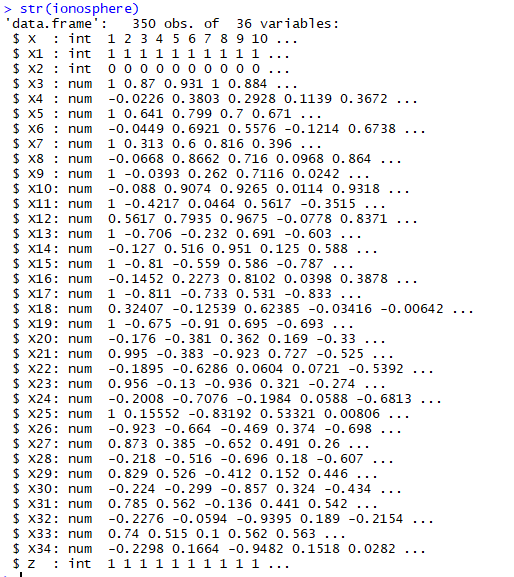
\includegraphics[scale = .5]{./discrimination/ionosphere/str.PNG} &
    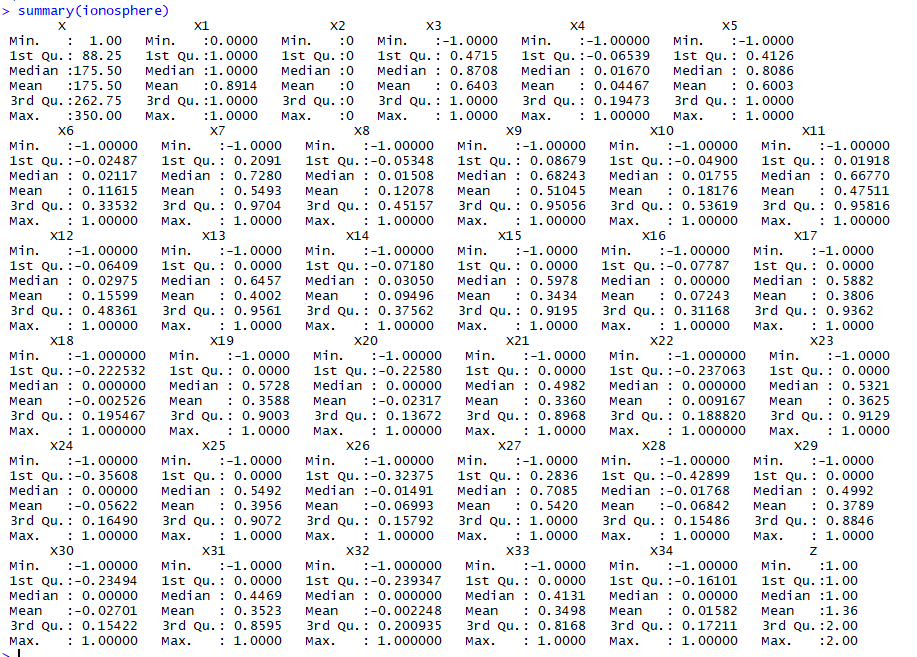
\includegraphics[scale = .5]{./discrimination/ionosphere/summary.PNG}
    \end{tabular}
    \caption{La strucutre du jeu de données \textbf{Ionosphere}}
    \label{fig:my_label}
\end{figure}
Nous pouvons voir que la variable \textit{X2} est toujours nulle dans ce jeu de données donc nous décidons de la supprimer. A partir des résultats ci-dessus, on peut voir que toutes les variables sont des variables numériques. Toutes les variables sont dans l'intervale [-1,1]. D'autre part, dans le but d'étudier la corrélation entre les variables qui peut produire des influences dans les méthodes de discrimination, nous avons un graphique chacun des variables. \newline
\begin{figure}[htb]
    \centering
    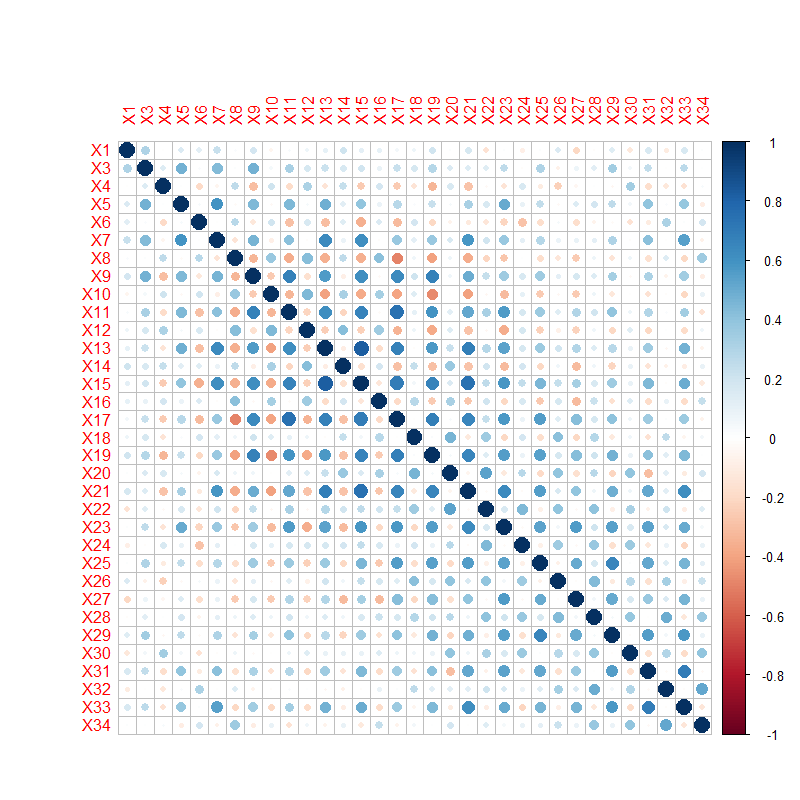
\includegraphics[scale = .4]{./discrimination/ionosphere/corrplot.png} 
    \caption{La corrélation entre les variables de \textbf{ionosphere}}
    \label{fig:my_label}
\end{figure}
Le test de corrélations a été réalisé par la méthode de Pearson avec \textbf{p-value} a été fixée par défault pour $\alpha = 0.05$. Grâce au graphique, on peut observer facilement qu'il y a des paires corrélé  comme $(X13,X5)$, $(X9,X17)$ mais la corrélation n'est pas très significative. L'étude de la corrélation est poursuivie par la réalisation d'analyse en composantes principales. Comme l'étude précédent, on veut au premier temps explorer la géométrie des données et à partir de cela, on peut prévoir le modèle compatible. \newline
Nous avons obtenu d'abord 2 graphiques : le cercle de corrélation et l'inertie de valeurs propres de 10 premières valeurs en utilisant la fonction \textit{princomp} et des fonctions du biliothèque \textit{factoextra}.
\begin{figure}[htb]
    \centering
    \begin{tabular}{c|c}
    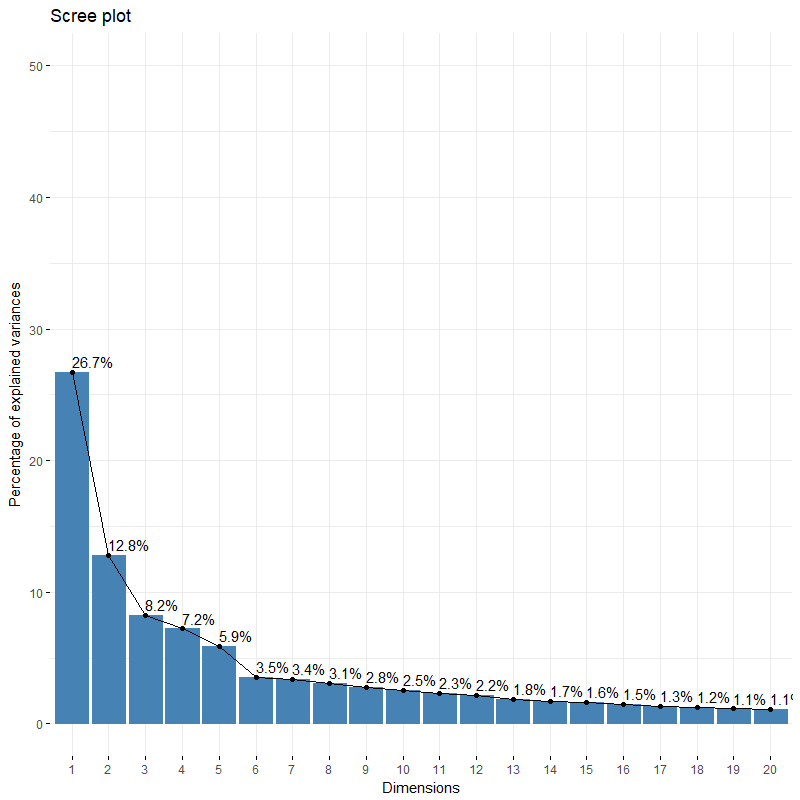
\includegraphics[scale = .3]{./discrimination/ionosphere/eigplot.png} &
    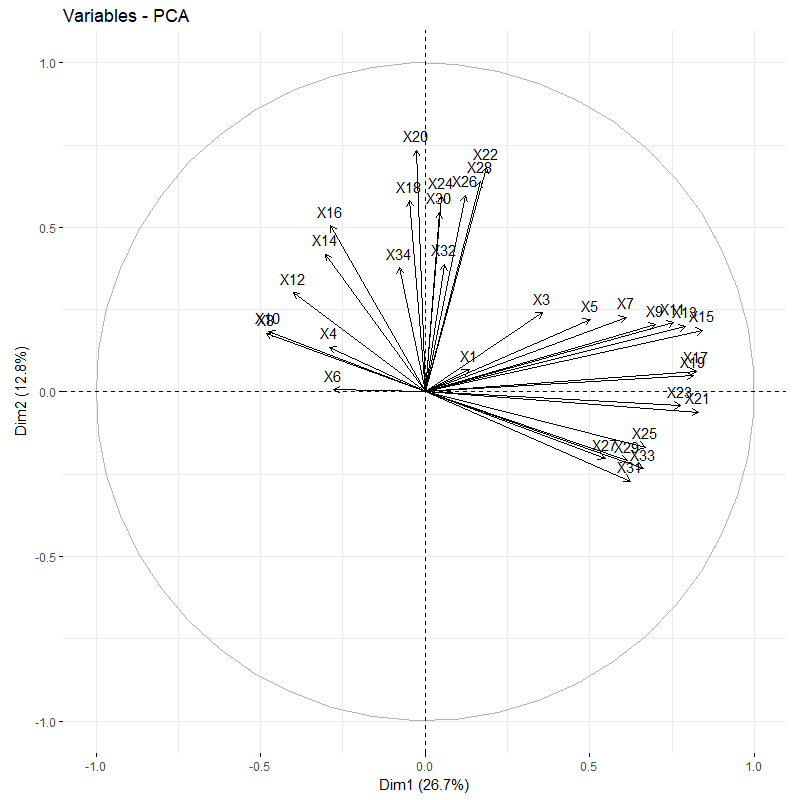
\includegraphics[scale = .3]{discrimination/ionosphere/variable_plot.png}
    \end{tabular}
    \caption{Graphique a : L'inertie de valeurs propres de 10 premières valeurs - Graphique b : Le cercle de corrélation des variables \textbf{breastcancer}}
    \label{fig:my_label}
\end{figure}
Dans le cadre de notre analyse, nous pouvons voir que les informations se concentrent aux 20 premières composantes avec plus de 90\% des informations totales. De plus, le cercle de corrélation des variables expliqué par les deux premières composantes nous montre la corrélation entre les variables. On peut vois dans le cercle de corrélation que les variables se séparent en 2 groupes principaux : un groupe ont tendance  au sens de la première composantes et un groupe ont tendance au sense de la deuxmième composantes. On observe la distribution des individus dans le graphique des individus ci-dessous : 
\begin{figure}[htb]
    \centering
    \begin{tabular}{cc}
    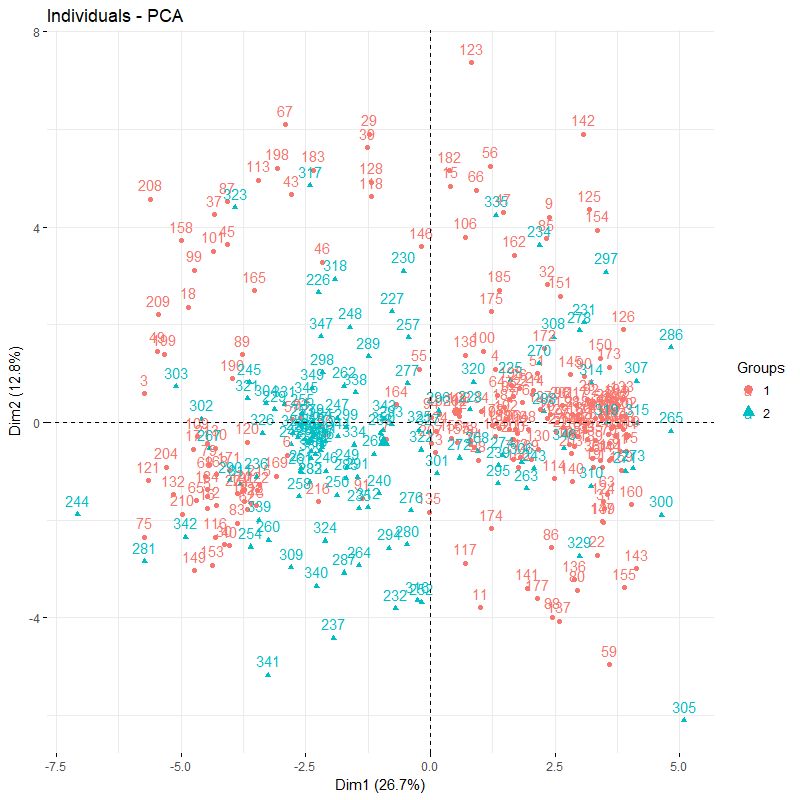
\includegraphics[scale = .3]{./discrimination/ionosphere/indi_plot12.png} &
    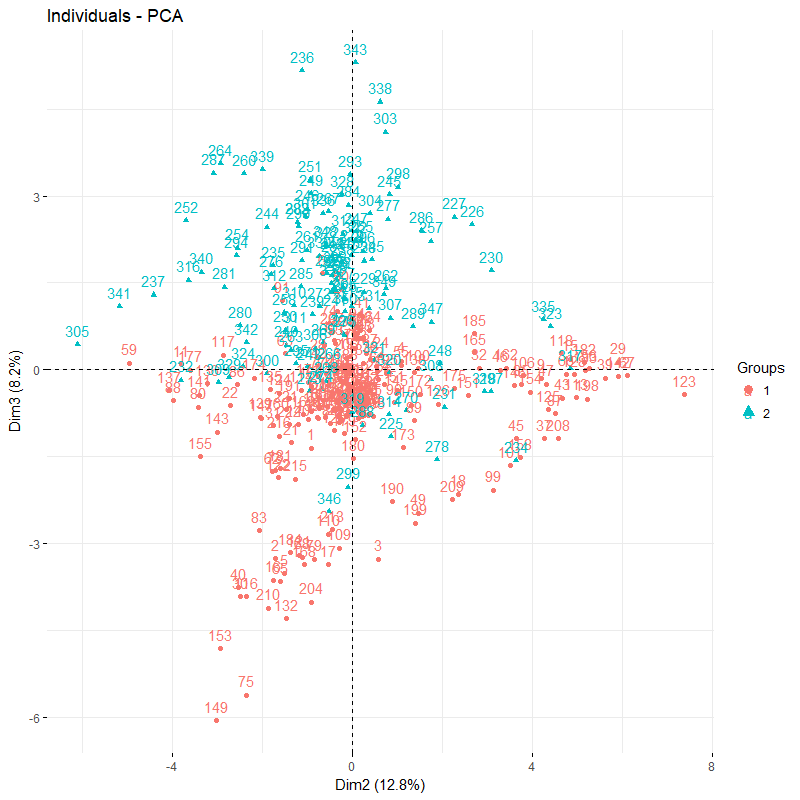
\includegraphics[scale = .3]{./discrimination/ionosphere/indi_plot23.png} 
    \end{tabular}
    \caption{La distribution des individus, graphique a : dans 2 premières composantes - graphique b : dans la 2eme et 3ème composante de \textbf{ionosphere}}
    \label{fig:my_label}
\end{figure}
La distribution des individus dans le graphique dans ce cas n'est plus très claire. Nous pouvons voir que dans la $2^{ème}$ et $3^{ème}$ composante principale, les individus sont plus séparés donc nous décidons de tracer le cercle de corrélation des variables dans ce plan.
\begin{figure}[htb]
    \centering
    \begin{tabular}{cc}
    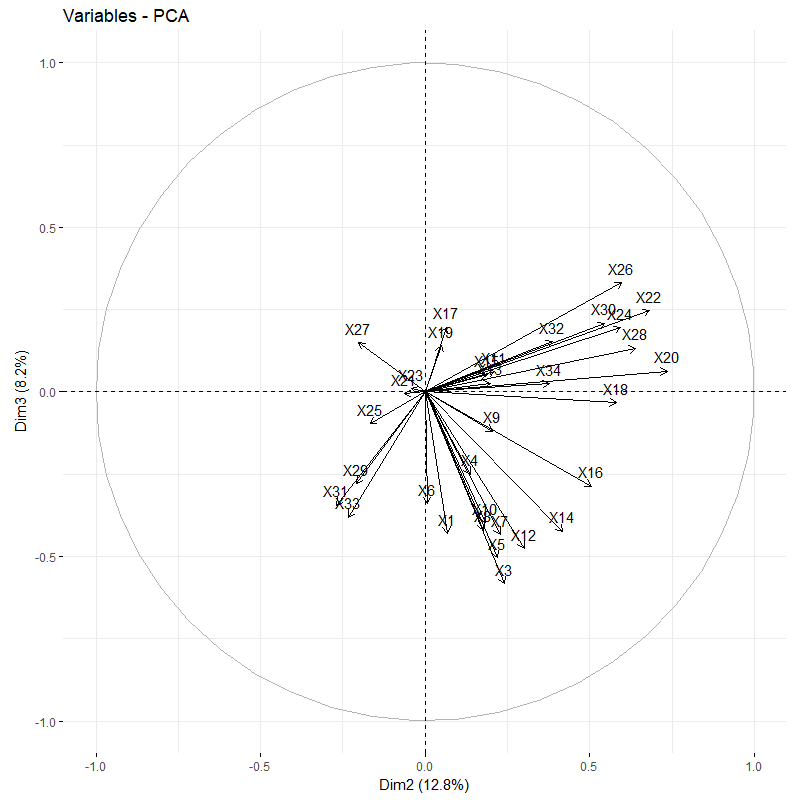
\includegraphics[scale = .3]{./discrimination/ionosphere/varplot23.png} 
    \end{tabular}
    \caption{Le cercle de corrélation des variables dans la 2eme et 3ème composante de \textbf{ionosphere}}
    \label{fig:my_label}
\end{figure}
La distribution des individus est maintenant un peu plus visible : les individus de classe 1 sont distribuées généralement au centre tandis que les individus de classe 2 se situent dans la partie positive de la $3^{ème}$ composante principale. Les deux classes ne sont pas séparées assez clairement pour une frontière linéaire donc nous pouvons prévoir que l'analyse de discriminante quadratique peut nous donner une classification plus précise dans ce cas. Pour la régression logistique, on a plus des variables mais moins d'individus donc il est difficile que la régression logistique nous donne un résultat intéressant avec les données non pré-traitées.  Pour vérifier notre prédiction, nous viendrons la réalisation des méthodes de discrimination sur ce jeu de données.
\subsubsection{Réalisation des méthode de discrimination}
Pour calculer le taux d'erreur ponctuelle $\Hat{\epsilon}$ d'une prédiction, il faut simplement compter le nombre de prédiction erronées $\epsilon_i$ entre la prédiction faite et les données réelle (d'apprentissage ou de test), puis diviser par le nombre total d'individus \textit{n}. \newline
On répète cette procédure 100 fois pour obtenir 100 réalisations du taux d'erreur. Pour obtenir l'estimation du taux d'erreur $\Bar{\epsilon}$, il ne reste plus qu'à faire la moyenne des 100 réalisations. \newline
L'intervalle de confiance à 95\% est obtenu comme-ci : $IC = \left[\mu - 1.96*\frac{s^{*}}{\sqrt{N}};\mu + 1.96*\frac{s^{*}}{\sqrt{N}} \right]$ avec : \newline
\begin{itemize}
    \item $\mu$ : La moyenne des 100 réalisation de $\epsilon$ \\
    \item $s^{*}$ : L'écart-type corrigé des 100 réalisations de $\epsilon$ \\
    \item $N$ : Le nombre de réalisation et dans ce cas $N=100$
\end{itemize}
Nous avons appliqué des différents modèles d'analyses discriminantes, de régression logistique ainsi que les arbres de décisions. Le résume des résultats sont en table ci-dessous.
\begin{table}[H]
\centering

\begin{tabular}{l|l|cc}
\multicolumn{1}{l|}{\textbf{Méthode}}    & \textbf{Données} &$ \overline{\varepsilon}$ & $IC$                      \\ \hline
\multirow{2}{*}{Analyse discriminante quadratique} & Apprentissage    &  0.0560                   & $\left[0.0542 ;~ 0.0578 \right]$  \\
                                       & Test             &  0.0285             & $\left[0.0258 ;~ 0.0312 \right]$ \\ \hline
\multirow{2}{*}{Analyse discriminante linéaire}                  & Apprentissage & 0.1089                                 & $\left[0.1618 ;~ 0.1113 \right]$  \\
                                       & Test             & 0.0891                       & $\left[0.0850  ;~ 0.0933 \right]$ \\ \hline
\multirow{2}{*}{Classifieur bayésien naïf}                  & Apprentissage    & 0.1661                             & $\left[0.1618 ;~ 0.1704 \right]$  \\
                                       & Test             & 0.1578                                 & $\left[0.1517 ;~ 0.1638 \right]$ \\ \hline
\multirow{2}{*}{Régression logistique (intercept=1)}                  & Apprentissage    & 0.0578                             & $\left[0.0549 ;~ 0.0606 \right]$  \\
                                       & Test             & 0.1235                                 & $\left[0.1179;~ 0.1290 \right]$ \\ \hline
\multirow{2}{*}{Régression logistique (intercept=0)}                  & Apprentissage    & 0.0549                           & $\left[0.0479 ;~ 0.0618 \right]$  \\
                                       & Test             & 0.1264                                & $\left[0.1095 ;~ 0.1433 \right]$ \\ \hline
\multirow{2}{*}{Arbre de décision}                  & Apprentissage    & 0.0686                             & $\left[0.0609 ;~  0.0763 \right]$  \\
                                       & Test             & 0.1239                                 & $\left[0.1064 ;~ 0.1414 \right]$ 
\end{tabular}

\caption{Calcul du taux d'erreur d'apprentissage $\varepsilon$ et de test pour le jeu de données ionosphere avec plusieurs méthodes (arrondi à $10^{-4})$}
\label{ionosphere}
\end{table}
On remarque ici que dans le cas de la régression logistique, on ne peut pas réaliser l'analyse sur le jeu de données initial comme nous avons prévu car dans certains cas nous obtenons ce résultat : $det(X^{T}W_{q}X) =  0$ donc il n'est pas possible d'inverser cette matrice. On crois que dans ce jeu de données, il y trop de paramètres à estimer, notamment dans le cas de régression logistique quadratique mais on n'a que 350 individus. Nous donc décidons d'utiliser l'ACP avec le fait que l'informations se concentrent aux 25 premières composantes avec plus de 90\%. La régression logistique se fonctionne bien après ce traitement mais la régression logistique quadratique nous donne toujours des erreurs. C'est reasonable parce que avec 25 variables à initial, après la transformation la dimension de notre données est de (350,350). C'est-à-dire on a moins que 350 individus pour l'apprentissage et il y a trop de paramètres. Nous continuons à diminuer le nombre de composantes jusqu'à 6 composantes. Mais avec 6 composantes principales, nous ne conservons pas beaucoup d'informations (50\%) donc la régression logistique quadratique n'est pas pratique dans ce cas. \newline
\begin{figure}[htb]
    \centering
    \begin{tabular}{cc}
    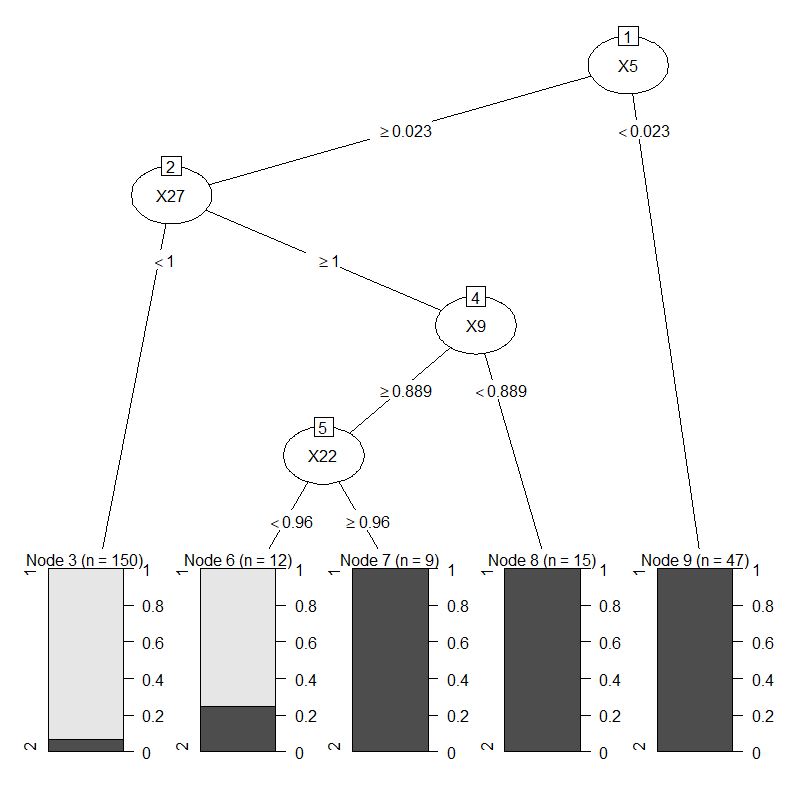
\includegraphics[scale = .4]{./discrimination/ionosphere/tree_plot.png} &
    \end{tabular}
    \caption{L'arbre de décision \textbf{breastcancer}}
    \label{fig:my_label}
\end{figure}
\newline
D'après la table \ref{ionosphere}, l'analyse discriminante quadratique permet d'obtenir les très bonnes même si avec donnéees initiales. Comme ce que nous avons analysé dans la partie de l'ACP, les individus ne sont pas séparés très clairement (il y a quelques individus d'un groupe se situent dans un autre groupe) donc nous avons besoin d'un modèle assez compliqué pour bien classifier les individus. Le classifieur bayésien naïf nous donne les taux d'erreurs assez forts car ce modèle est trop simple pour expimer ce jeu de données. l'analyse discriminante linéaire peut nous donner un resultat acceptable car ce modèle est plus robuste que le classifieur bayésien naïf. Les resultats obtenus par la régression logistique et arbre de décision sont plus grands que l'analyse discriminante linéaire mais ils sont acceptables. On remarque ici que \textit{overfitting} apparait dans le cas de la régresssion logistique et l'arbre de décision parce qu'on a peu de données dans ce jeu de données. La régression logistique est robuste mais il faut avoir plusieurs de données pour stabiliser ce modèle. On note également ici que l'ajout de l'ordonnée à l'origine  n'est pas éfficace car il n'y a pas beacoup de valeur nulle dans ce jeu de données (9\%) et la valeur maximale de chaque variable est $1$. Plus généralement, les classifieurs se basant sur la distribution gaussienne ont de très bons résultats sur ces données car cela correspond effectivement à la vraie distribution des données.


\subsection{Sonar}
\subsubsection{Analyse exploratoire}
Comme le jeu de données précédent, nous avons d'abord effectué une analyse exploratoire pour comprendre et s'approcher les données fournies. \newline
Ce jeu de données comporte 60 variables et 208 individus. On a exclu la première colonne parce que cela correspond à l'index qui est inutile dans notre analyse.
\begin{figure}[htb]
    \centering
    \begin{tabular}{cc}
    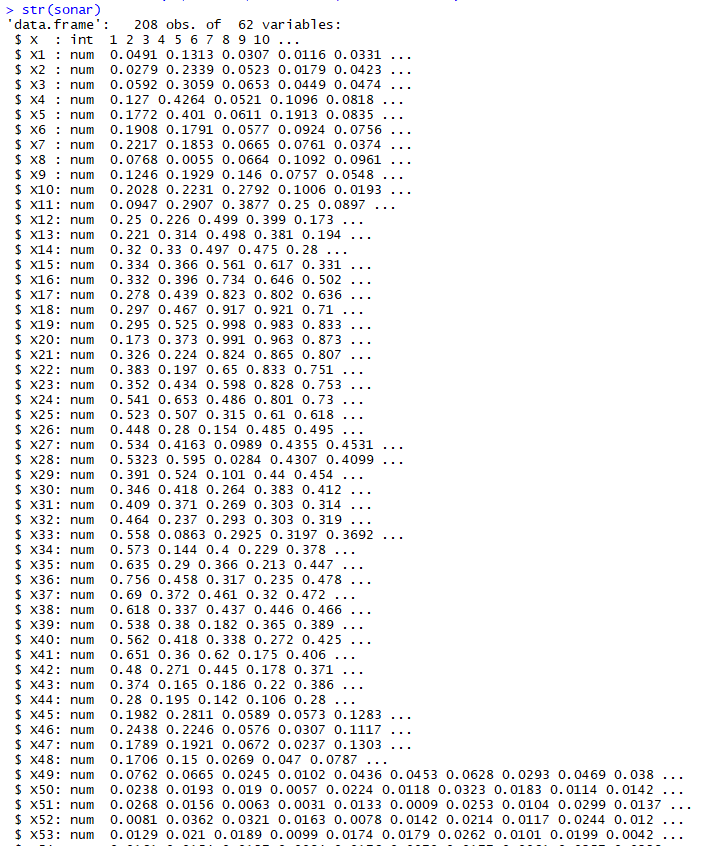
\includegraphics[scale = .5]{./discrimination/Sonar/str.PNG} &
    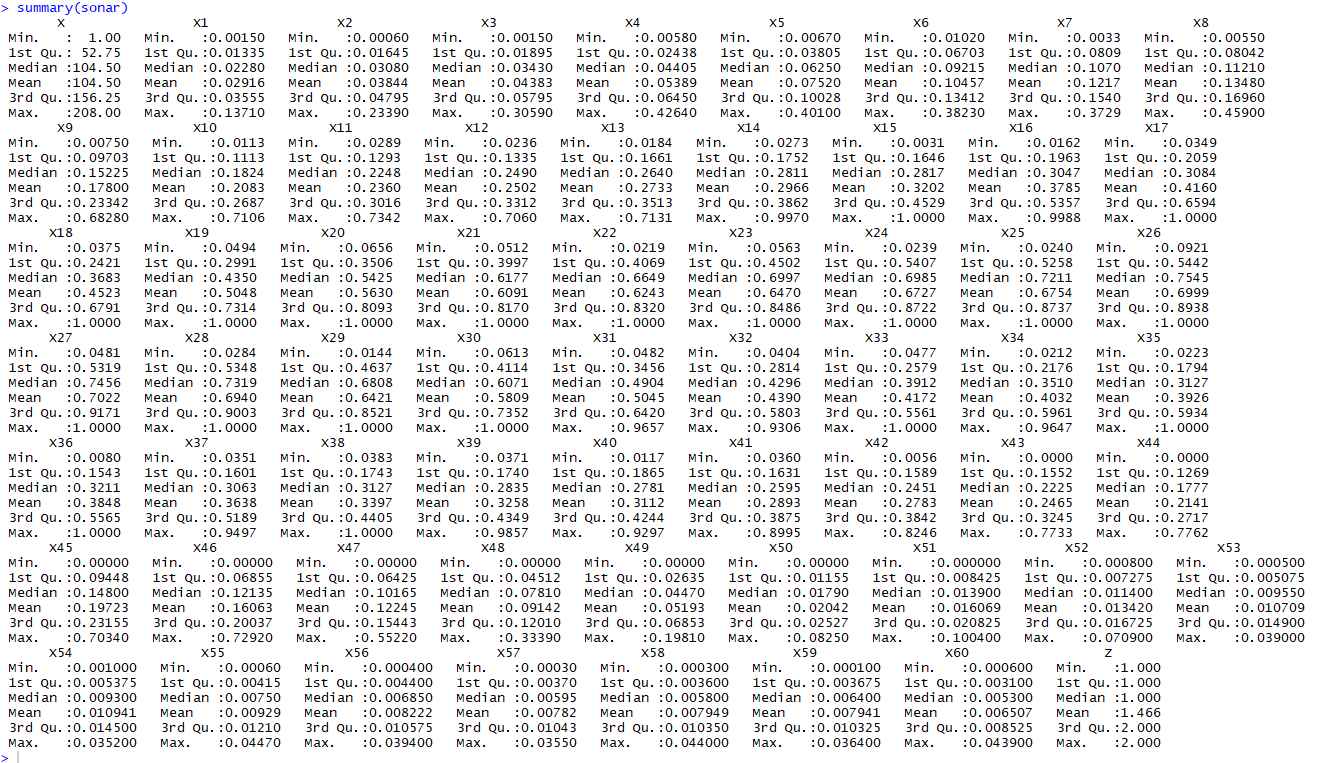
\includegraphics[scale = .3]{./discrimination/Sonar/summary.PNG}
    \end{tabular}
    \caption{La strucutre du jeu de données \textbf{Sonar}}
    \label{fig:my_label}
\end{figure}
A partir des résultats ci-dessus, on peut voir que toutes les variables sont des variables numériques. Toutes les variables sont dans l'intervale [0,1]. Nous pouvons voir d'abord que ce jeu de données comporte très peu des individus et beaucoup de variables. Ce sera difficile à appliquer les méthodes qui ont besoin de plusieurs données pour stabiliser le modèle comme la régression ou les méthodes qui doivent estimer beaucoup de paramètres comme l'analyse discriminante quadratique. On croit que \textbf{overfitting} apparaîtrait dans plupart des analyses. On puis étudie la corrélation des variables.
\newline
\begin{figure}[htb]
    \centering
    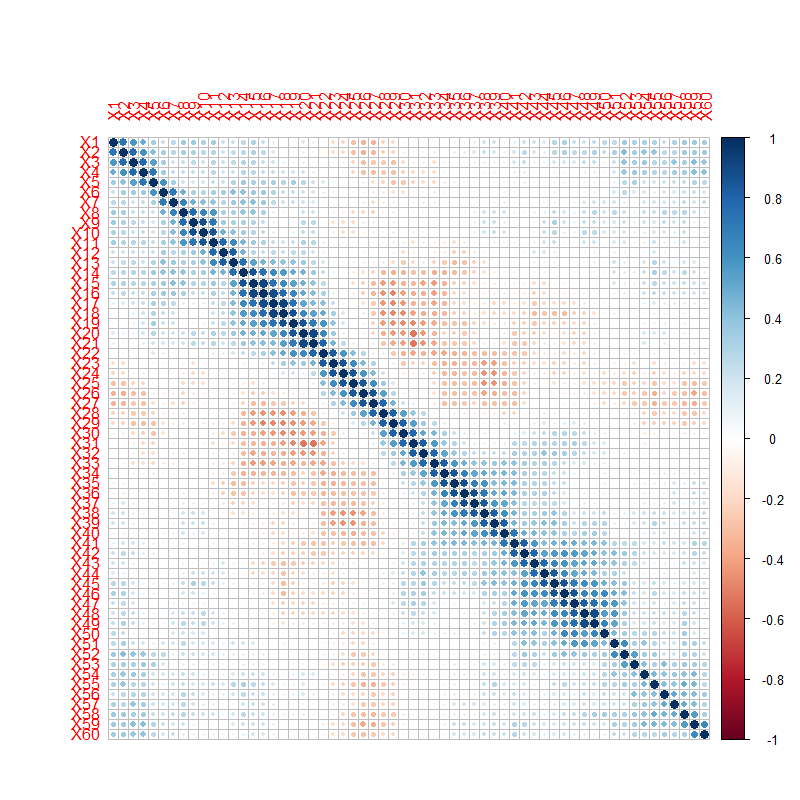
\includegraphics[scale = .4]{./discrimination/Sonar/corrplot.png} 
    \caption{La corrélation entre les variables de \textbf{Sonar}}
    \label{my_label}
\end{figure}
Le test de corrélations a été réalisé par la méthode de Pearson avec \textbf{p-value} a été fixée par défault pour $\alpha = 0.05$. Grâce au graphique, on peut observer la corrélation entre des variables n'est pas significative sauf les points autour de la diagonale principale. C'est-à-dire que les variables sont corrélé avec les variables "voisines". L'étude de la corrélation est poursuivie par la réalisation d'analyse en composantes principales. Comme l'étude précédent, on veut au premier temps explorer la géométrie des données et à partir de cela, on peut prévoir le modèle compatible. \newline
Nous avons obtenu d'abord 2 graphiques : le cercle de corrélation et l'inertie de valeurs propres de 10 premières valeurs en utilisant la fonction \textit{princomp} et des fonctions du biliothèque \textit{factoextra}.
\begin{figure}[htb]
    \centering
    \begin{tabular}{c|c}
    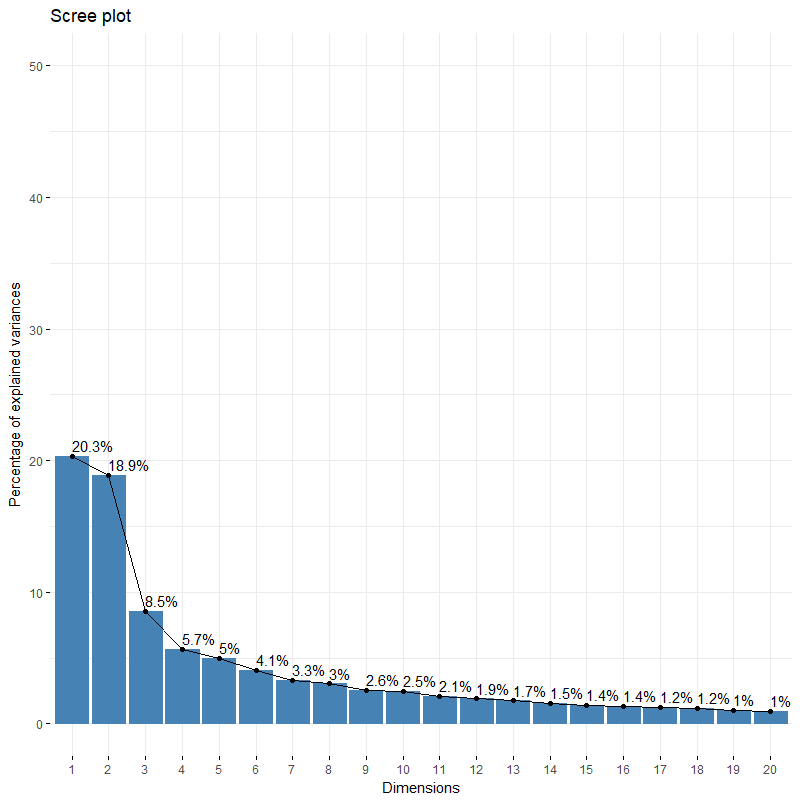
\includegraphics[scale = .3]{./discrimination/Sonar/eig_plot.png} &
    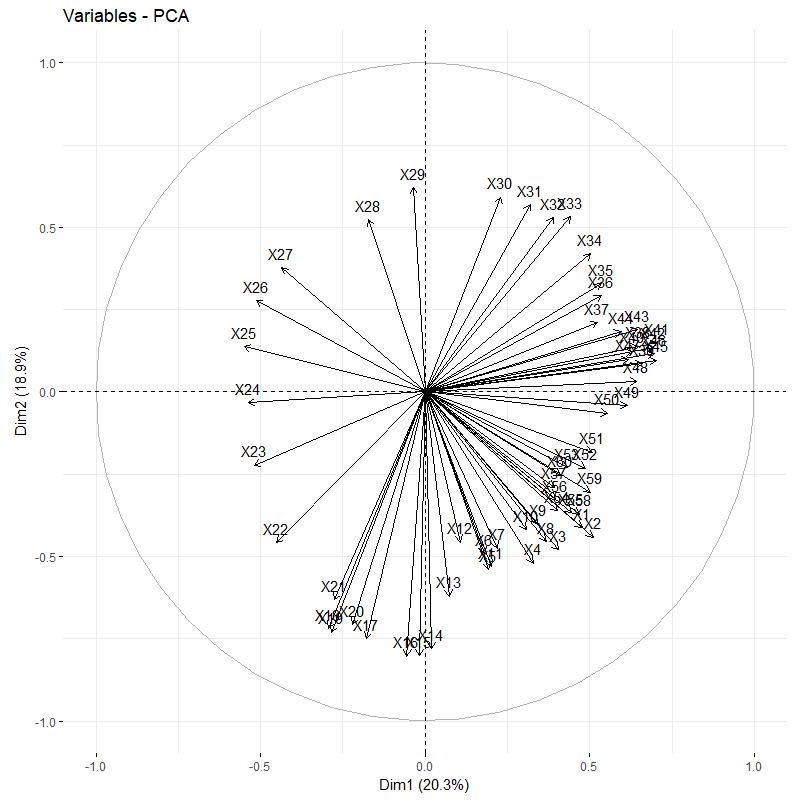
\includegraphics[scale = .3]{discrimination/Sonar/var_plot.png}
    \end{tabular}
    \caption{Graphique a : L'inertie de valeurs propres de 10 premières valeurs - Graphique b : Le cercle de corrélation des variables \textbf{Sonar}}
    \label{fig:my_label}
\end{figure}
Dans le cadre de notre analyse, nous pouvons voir que les informations se concentrent aux 25 premières composantes avec plus de 92\% des informations totales. De plus, le cercle de corrélation des variables expliqué par les deux premières composantes nous montre la corrélation entre les variables. On observe la distribution des individus dans le graphique des individus ci-dessous. 
\begin{figure}[htb]
    \centering
    \begin{tabular}{ccc}
    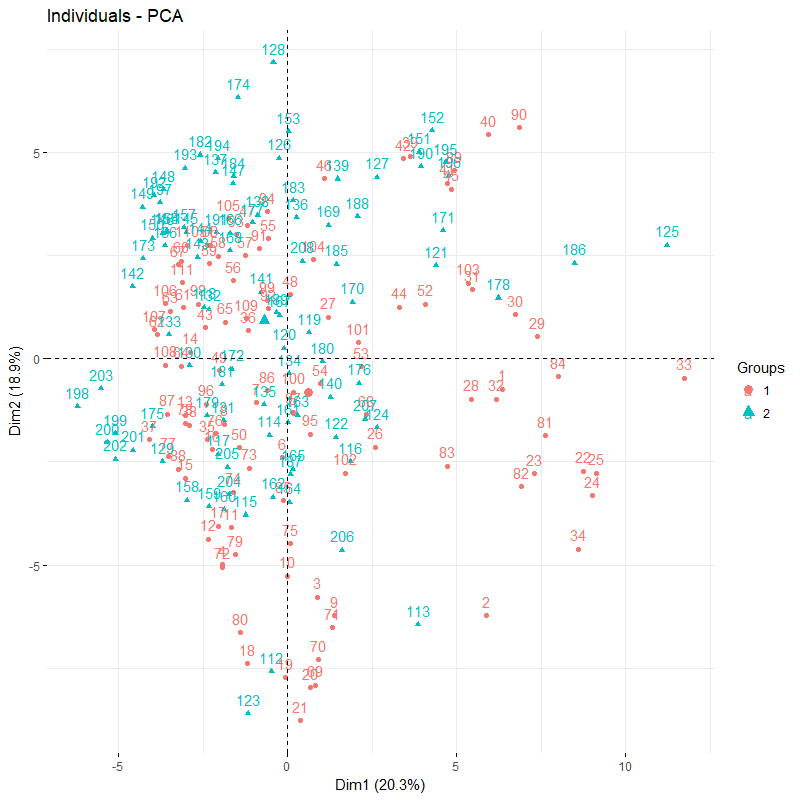
\includegraphics[scale = .3]{./discrimination/Sonar/indi_plot12.png} &
    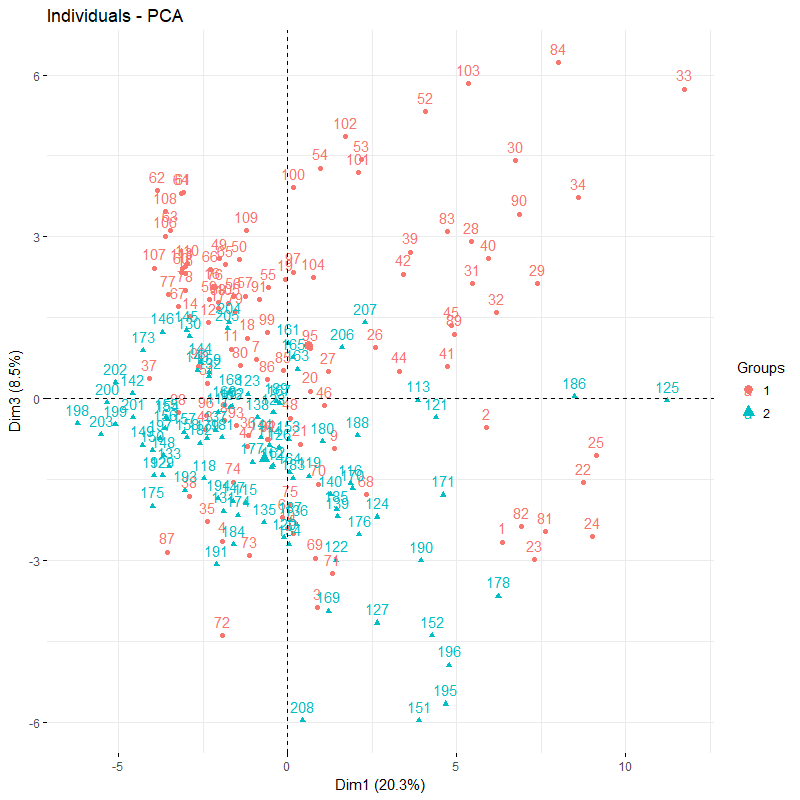
\includegraphics[scale = .3]{./discrimination/Sonar/indi_plot13.png} 
    \end{tabular}
    \caption{La distribution des individus, graphique a : dans 2 premières composantes - graphique b : dans la 1me et 3ème composante \textbf{Sonar}}
    \label{fig:my_label}
\end{figure}
\newline
La distribution des individus dans le graphique dans ce cas n'est plus très claire. Nous pouvons voir que dans la $1^{ère}$ et $3^{ème}$ composante principale, les individus sont plus séparés donc nous décidons de tracer le biplot dans ce plan. \newline
\begin{figure}[htb]
    \centering
    \begin{tabular}{ccc}
    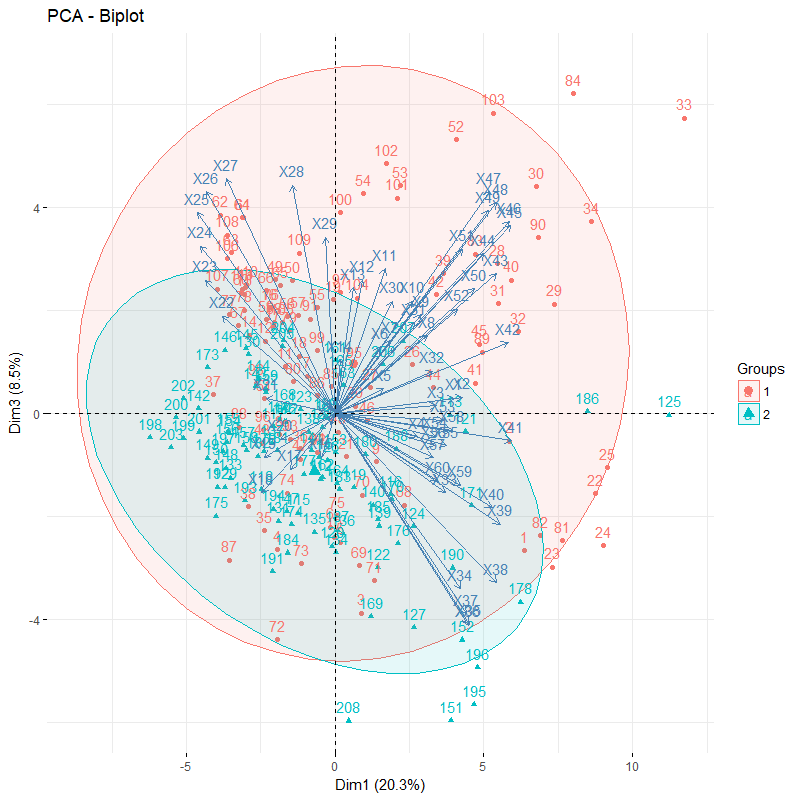
\includegraphics[scale = .3]{./discrimination/Sonar/biplot13.png}  
    \end{tabular}
    \caption{Biplot dans la 1me et 3ème composante \textbf{Sonar}}
    \label{fig:my_label}
\end{figure}
La relation entre les variables et les individus est maintenant un peu plus visible : les individus de classe 1 ont tendance de distribuer généralement selon les variables tandis que les individus de classe 2 ne l'ont pas. Les deux classes ne sont pas séparées assez clairement pour une frontière linéaire donc nous pouvons prévoir que l'analyse de discriminante quadratique peut nous donner une classification plus précise mais dans ce cas pour obtenir les résultats sans \textit{overfitting}, il faut pré-traiter ce jeu de données. Avec ce jeu de données peu d'individus comme \textbf{Sonar}, le classifieur bayésien naïf peut se fonctionner bien mais dans ce cas, la distribution des individus est compliquée pour que un modèle simple comme le classifieur bayésien naïf puisse nous donner un résultat agréable. Pour vérifier notre prédiction, nous viendrons la réalisation des méthodes de discrimination sur ce jeu de données.
\subsubsection{Réalisation des méthode de discrimination}
Pour calculer le taux d'erreur ponctuelle $\Hat{\epsilon}$ d'une prédiction, il faut simplement compter le nombre de prédiction erronées $\epsilon_i$ entre la prédiction faite et les données réelle (d'apprentissage ou de test), puis diviser par le nombre total d'individus \textit{n}. \newline
On répète cette procédure 100 fois pour obtenir 100 réalisations du taux d'erreur. Pour obtenir l'estimation du taux d'erreur $\Bar{\epsilon}$, il ne reste plus qu'à faire la moyenne des 100 réalisations. \newline
L'intervalle de confiance à 95\% est obtenu comme-ci : $IC = \left[\mu - 1.96*\frac{s^{*}}{\sqrt{N}};\mu + 1.96*\frac{s^{*}}{\sqrt{N}} \right]$ avec : \newline
\begin{itemize}
    \item $\mu$ : La moyenne des 100 réalisation de $\epsilon$ \\
    \item $s^{*}$ : L'écart-type corrigé des 100 réalisations de $\epsilon$ \\
    \item $N$ : Le nombre de réalisation et dans ce cas $N=100$
\end{itemize}
Comme nous avons discuté dessus, il est difficile à analyser ce jeu de données sans \textit{overfitting} donc nous d'abord pré-traitons ce jeu de données par la méthode l'ACP comme d'habitude. Nous choisissons 25 premières composantes principales qui nous permettent de conserver plus de 92\% de l'informations. \\
Nous avons puis appliqué des différents modèles d'analyses discriminantes, de régression logistique ainsi que les arbres de décisions. Le résume des résultats sont en table ci-dessous.
\begin{table}[H]
\centering

\begin{tabular}{l|l|cc}
\multicolumn{1}{l|}{\textbf{Méthode}}    & \textbf{Données} &$ \overline{\varepsilon}$ & $IC$                      \\ \hline
\multirow{2}{*}{Analyse discriminante quadratique} & Apprentissage    & 0.0470                   & $\left[0.0434 ;~ 0.0506 \right]$  \\
                                       & Test             & 0.2752             & $\left[0.2663  ;~ 0.2840 \right]$ \\ \hline
\multirow{2}{*}{Analyse discriminante linéaire}                  & Apprentissage & 0.1476                                 & $\left[0.1430 ;~ 0.1522 \right]$  \\
                                       & Test             & 0.2560                       & $\left[0.2470  ;~0.2651 \right]$ \\ \hline
\multirow{2}{*}{Classifieur bayésien naïf}                  & Apprentissage    &  0.1976                             & $\left[0.1897 ;~ 0.2056 \right]$  \\
                                       & Test             & 0.3136                                 & $\left[0.3035 ;~ 0.3236 \right]$ \\ \hline
\multirow{2}{*}{Régression logistique (intercept=1)}                  & Apprentissage    &  0.1223                             & $\left[ 0.1164 ;~ 0.1281 \right]$  \\
                                       & Test             & 0.2444                                 & $\left[0.2361;~ 0.2527 \right]$ \\ \hline
\multirow{2}{*}{Régression logistique (intercept=0)}                  & Apprentissage    &  0.1349                           & $\left[0.1297 ;~ 0.1401 \right]$  \\
                                       & Test             & 0.2486                                & $\left[0.2386 ;~ 0.2587 \right]$ \\ \hline
\multirow{2}{*}{Arbre de décision}                  & Apprentissage    &  0.1136                             & $\left[0.0978 ;~  0.1295 \right]$  \\
                                       & Test             & 0.2594                                 & $\left[0.2342 ;~ 0.2846 \right]$ 
\end{tabular}

\caption{Calcul du taux d'erreur d'apprentissage $\varepsilon$ et de test pour le jeu de données sonar avec plusieurs méthodes (arrondi à $10^{-4})$}
\label{sonar}
\end{table}
\begin{figure}[htb]
    \centering
    \begin{tabular}{cc}
    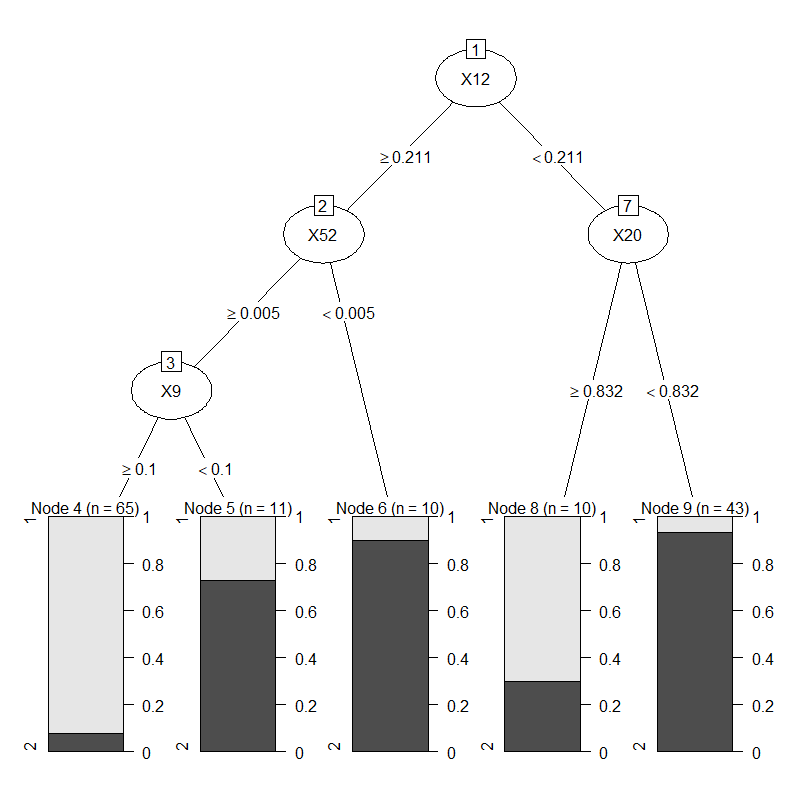
\includegraphics[scale = .4]{./discrimination/Sonar/tree_plot.png} &
    \end{tabular}
    \caption{L'arbre de décision \textbf{Sonar}}
    \label{fig:my_label}
\end{figure}
On remarque ici que dans le cas de la régression logistique quadratique, on ne peut pas réaliser l'analyse sur le jeu de données car dans certains cas nous obtenons ce résultat : $det(X^{T}W_{q}X) =  0$ donc il n'est pas possible d'inverser cette matrice. C'est reasonable parce que avec 25 variables à initial, après la transformation la dimension de notre données est de (207,350). C'est-à-dire on a moins que 350 individus pour l'apprentissage et c'est évidemment impossible. Nous continuons à diminuer le nombre de composantes jusqu'à 4 composantes. Mais avec 6 composantes principales, nous ne conservons pas beaucoup d'informations (53\%) donc la régression logistique quadratique n'est pas pratique dans ce cas. 
\newline
D'après la table \ref{sonar}, la régression logistique nous donne les meilleurs résultats. Comme ce que nous avons analysé dans la partie de l'ACP, les individus ne sont pas séparés très clairement (il y a beaucoup individus d'un groupe se situent dans un autre groupe) donc nous avons besoin d'un modèle assez flexible pour bien classifier les individus. Le classifieur bayésien naïf nous donne les taux d'erreurs assez forts car ce modèle est trop simple pour expimer ce jeu de données. L'analyse discriminante linéaire peut nous donner un resultat acceptable car ce modèle est plus robuste que le classifieur bayésien naïf. On remarque ici que \textit{overfitting} apparait dans plupart de cas comme nous avons prévu malgé au pré-traitement de données, parce qu'on a peu de données dans ce jeu de données. L'analyse discriminante quadratique est le cas de \textbf{overfitting} le plus visble cas le taux d'erreur d'apprentissage est 0.047 mais le taux d'erreur de test est beaucoup plus significatif. L'analyse discriminante quadratique est flexible donc dans certains cas, il peut "apprendre" facilement des bruits.La régression logistique est robuste mais il faut avoir plusieurs de données pour stabiliser ce modèle. Donc le pré-traitement de données par l'ACP ne peut pas résoudre completement le problème de \textit{overfitting}.  On note également ici que l'ajout de l'ordonnée à l'origine  augmente un peu l'efficace car la précision de la régression logistique dans le cas l'ajout de l'ordonnée à l'origine est un peu plus haute. Mais l'efficacement n'est pas très remarquable. L'arbre de décision n'améliore pas le résultat après le pré-traitement des données cas l'arbre de décision est une méthode non paramétrique donc elle est très sensible. Plus généralement, dans ce jeu de données, nous avons rencontré le problème \textit{overfitting}. Le problème est la conséquence de le fait que on a peu de données pour l'apprentissage. Nous avons essayé d'appliquer l'ACP pour résoudre ce problème. Le \textit{overfitting} diminue après le pré-traitement de données mais les taux d'erreur restent très significatifs. 




\subsection{Spambase}
\subsubsection{Analyse exploratoire}
Comme le jeu de données précédent, nous avons d'abord effectué une analyse exploratoire pour comprendre et s'approcher les données fournies. \newline
Ce jeu de données comporte 57 variables et 4601 individus. On a exclu la première colonne parce que cela correspond à l'index qui est inutile dans notre analyse.
\begin{figure}[htb]
    \centering
    \begin{tabular}{cc}
    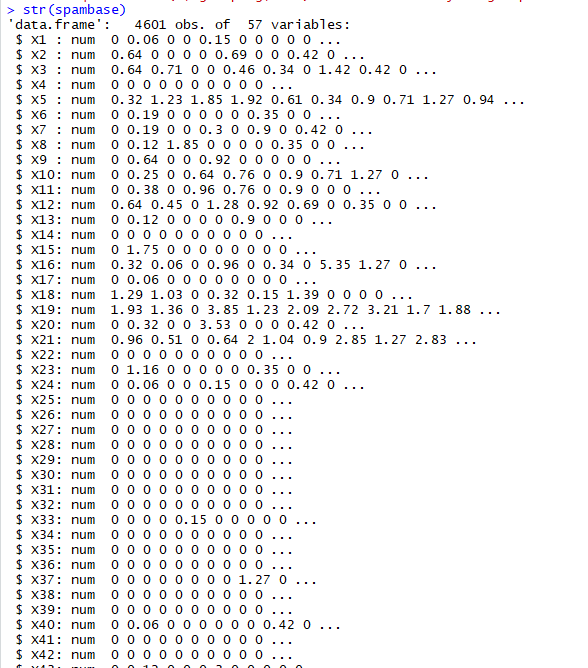
\includegraphics[scale = .5]{./discrimination/spambase/str.PNG} &
    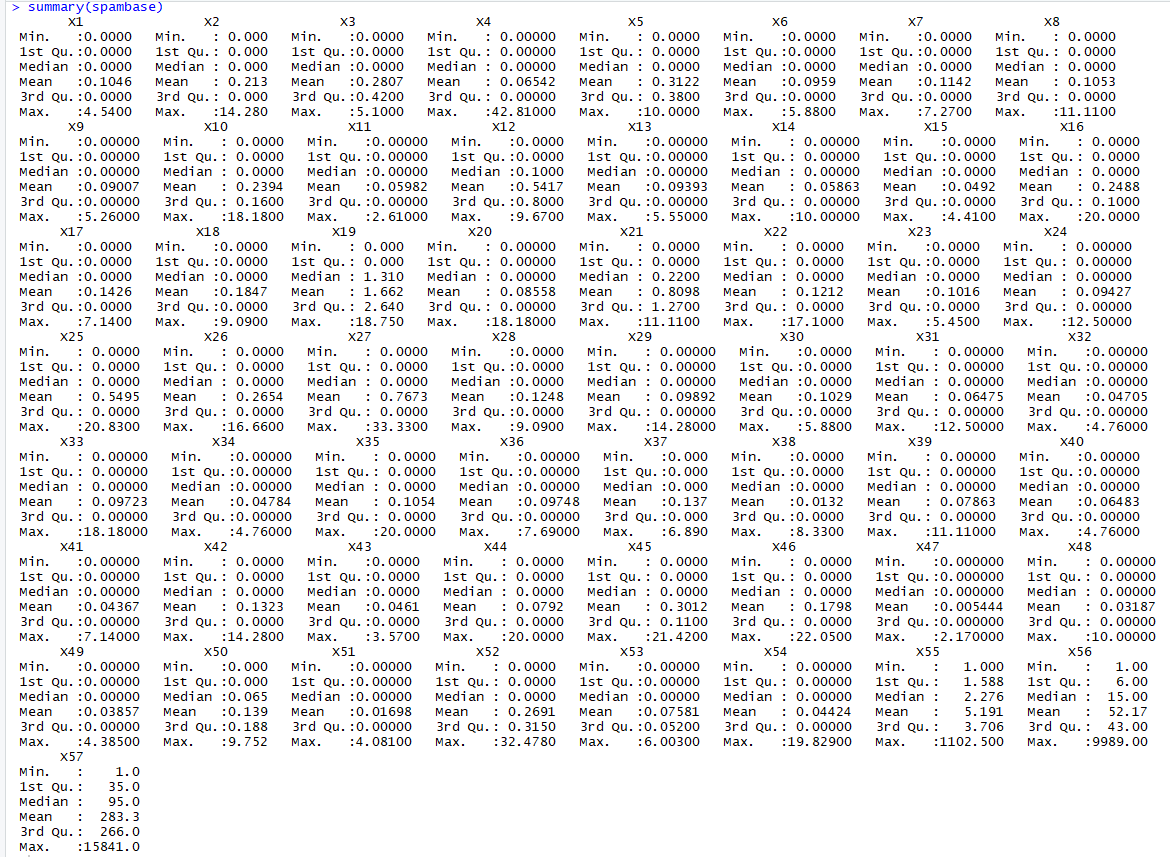
\includegraphics[scale = .3]{./discrimination/spambase/summary.PNG}
    \end{tabular}
    \caption{La strucutre du jeu de données \textbf{spambase}}
    \label{fig:my_label}
\end{figure}
A partir des résultats ci-dessus, on peut voir que toutes les variables sont des variables numériques. On remarque ici qu'il y a quelques variables ayant les valeurs très dominantes que les autres par exemple $X49$, $X55$, $X56$, $X57$. Nous donc voulons savoir si la covariance entre les variables est grande ou non. Après avoir étudié la covariance, on trouve qu'il y a 9 paires de variables dont les covariances sont suppérieures à 1000, 4 paires de variables dont les covariances sont suppérieur à 10000 et une paire dont la covariance est suppérieur à 100000. On puis étudie la corrélation des variables.
\newline
\begin{figure}[htb]
    \centering
    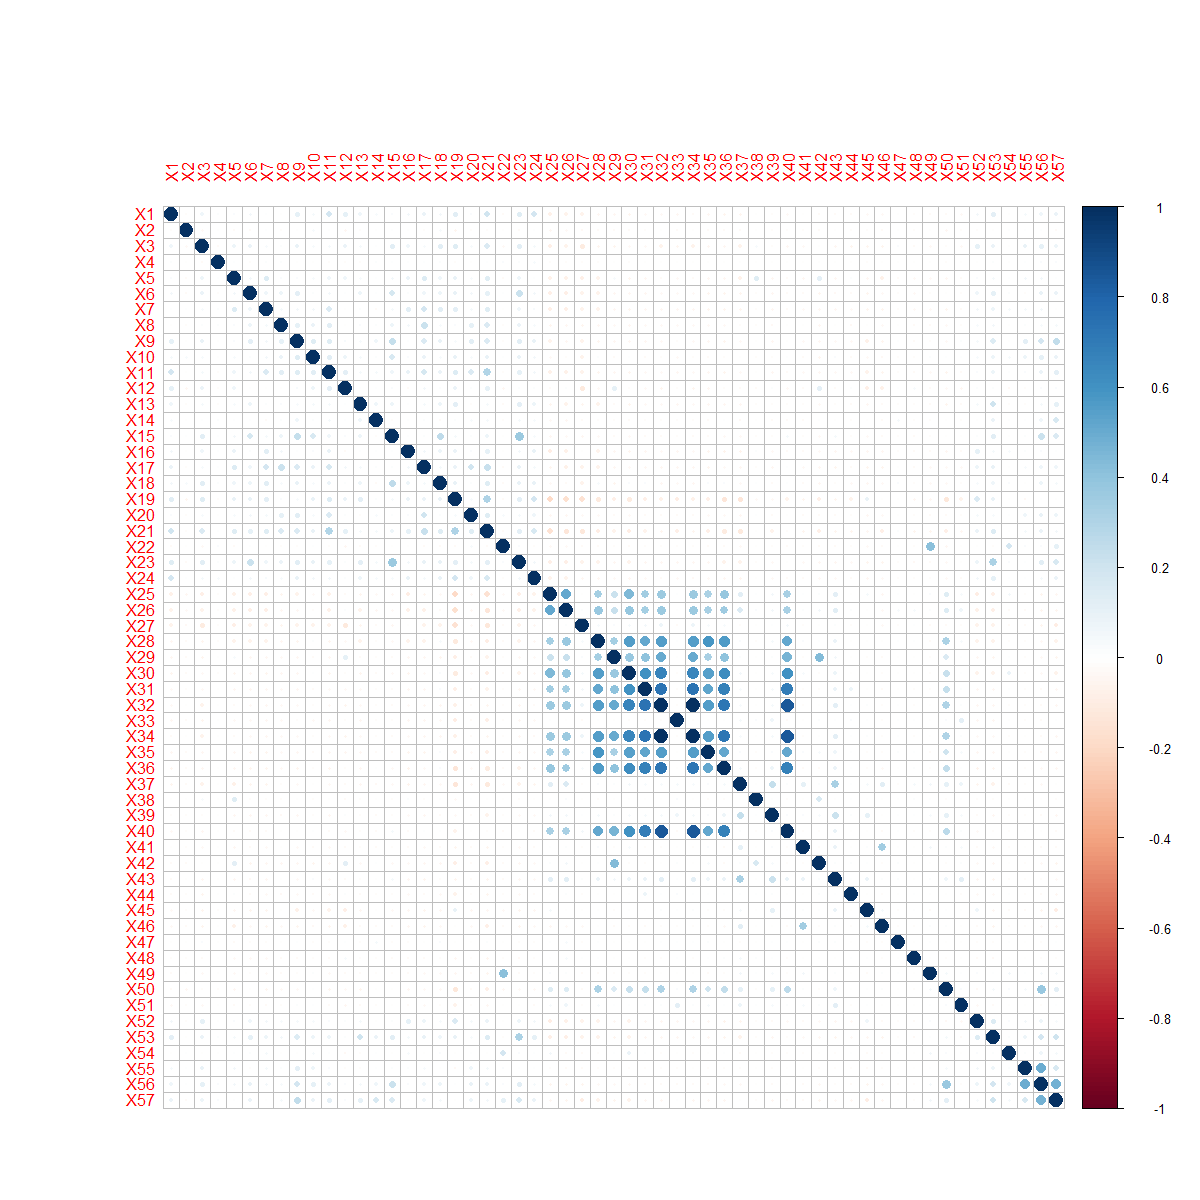
\includegraphics[scale = .4]{./discrimination/spambase/corrplot.png} 
    \caption{La corrélation entre les variables de \textbf{spambase}}
    \label{my_label}
\end{figure}
Le test de corrélations a été réalisé par la méthode de Pearson avec \textbf{p-value} a été fixée par défault pour $\alpha = 0.05$. Grâce au graphique, on peut observer la corrélation entre des variables n'est pas significative sauf $(X32,X34)$, $(X32,X40)$. C'est-à-dire que la plupart de variables sont indépendantes l'une à l'autre. Ce sera peut-être problèmatique pour notre analyse parce que dans nos analyses discriminantes quadratique et linéaire et le classifieur bayésien naïf, nous avons supposé que les vecteurs de caractéristique suit une loi normale multidimensionnelle.
\begin{equation}
    f_k(x) = \frac{1}{(2\pi)^{p/2}(det\Sigma_k)^{1/2}}exp\left( -\frac{1}{2}(x-\mu_k)^{T}\Sigma_k^{-1}(x-\mu_k)\right)
\end{equation}
A quelques points où la valeur est grande, s'ils sont indépendants l'un à l'autre et ses covariances sont grandes, le terme $-\frac{1}{2}(x-\mu_k)^{T}\Sigma_k^{-1}(x-\mu_k)$ peut devenir très petite, donc $exp\left( -\frac{1}{2}(x-\mu_k)^{T}\Sigma_k^{-1}(x-\mu_k)\right)$ sera approximatement égal à 0 et donc $f_k$ sera égale à 0. Si $f_k$ est égal à 0, la densité de mélange devient 0 et la probabilité a posteriori devient indéfinie car on ne peut pas diviser 0 par 0. Avec l'analyse ci-dessus, on croit qu'il y aurais quelque problèmes avec notre analyse discriminante. \newline
L'étude de la corrélation est poursuivie par la réalisation d'analyse en composantes principales. Comme l'étude précédent, on veut au premier temps explorer la géométrie des données et à partir de cela, on peut prévoir le modèle compatible. \newline
Nous avons obtenu d'abord 2 graphiques : le cercle de corrélation et l'inertie de valeurs propres de 10 premières valeurs en utilisant la fonction \textit{princomp} et des fonctions du biliothèque \textit{factoextra}.
\begin{figure}[htb]
    \centering
    \begin{tabular}{c|c}
    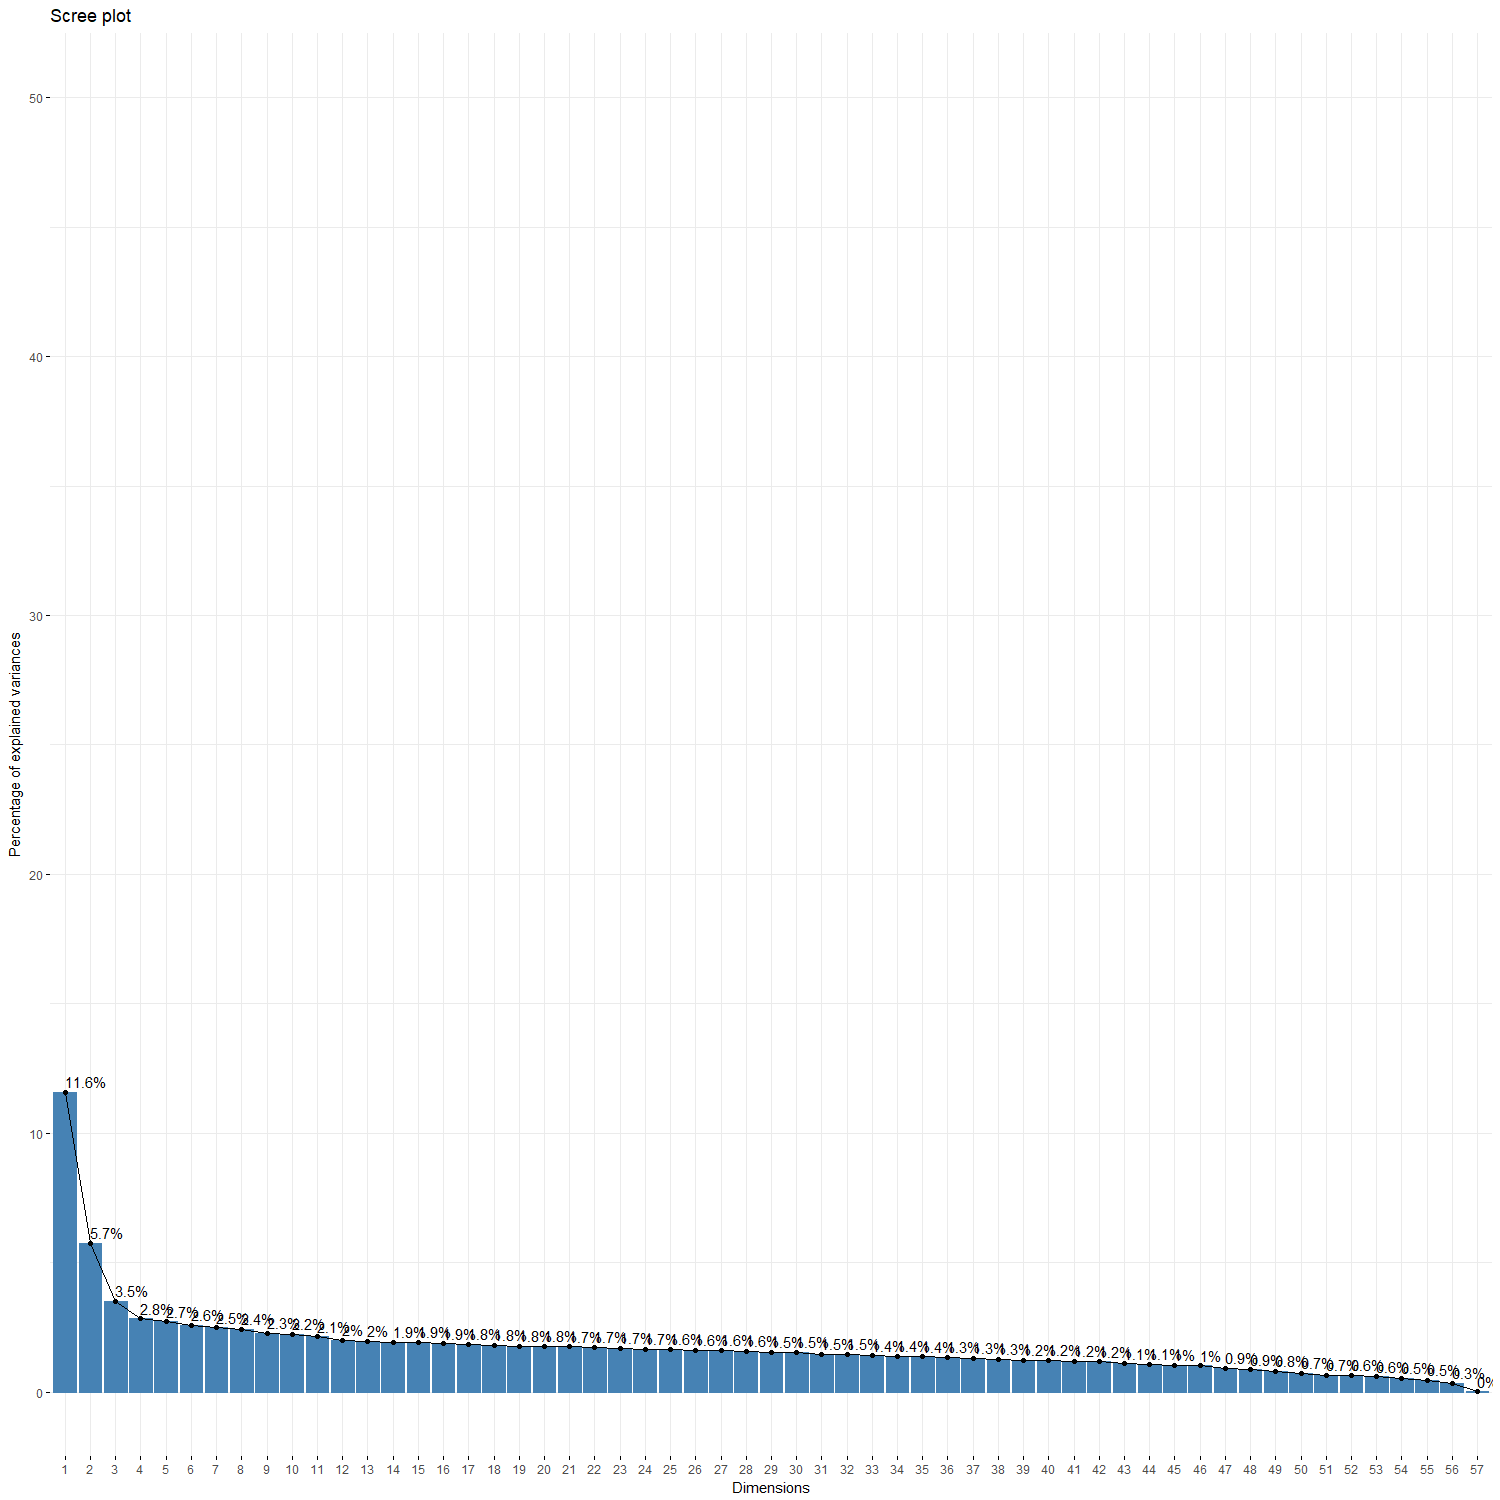
\includegraphics[scale = .2]{./discrimination/spambase/eig_plot.png} &
    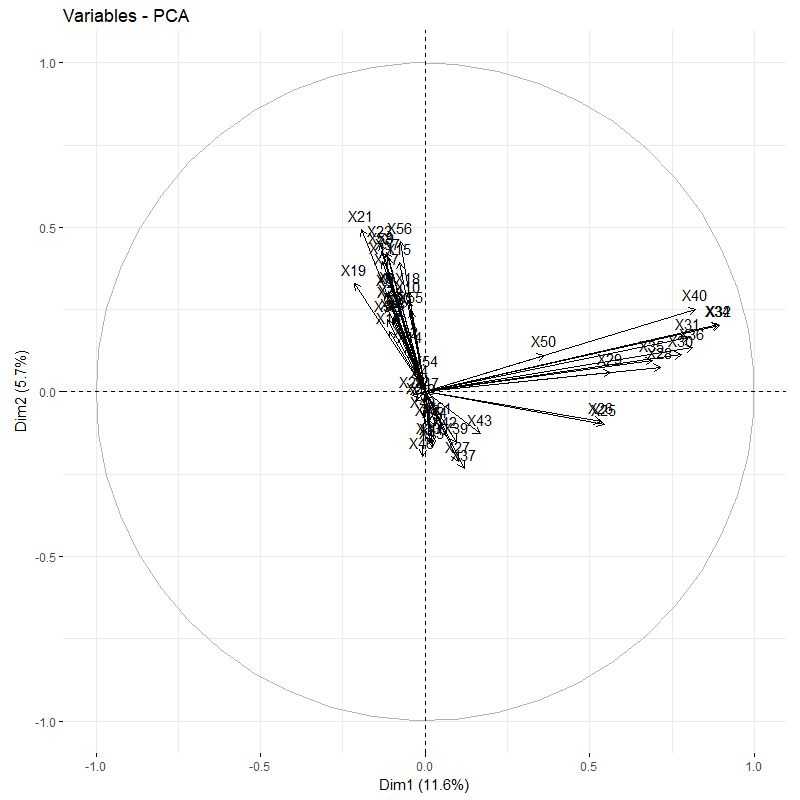
\includegraphics[scale = .3]{discrimination/spambase/var_plot.png}
    \end{tabular}
    \caption{Graphique a : L'inertie de valeurs propres de 10 premières valeurs - Graphique b : Le cercle de corrélation des variables \textbf{spambase}}
    \label{fig:my_label}
\end{figure}
Dans le cadre de notre analyse, nous pouvons voir que les informations se distribuent uniforement et 95\% de données se concentrent aux 45 premères composantes principales. C'est un autre problème de notre analyse car si on veut effectuer une diminuation de dimension par l'ACP, on doit choisir beaucoup de composantes pour conserver plupart de l'informations. Le cercle de corrélation des variables expliqué par les deux premières composantes nous montre la corrélation entre les variables. On observe la distribution des individus dans le graphique des individus ci-dessous. 
\begin{figure}[htb]
    \centering
    \begin{tabular}{ccc}
    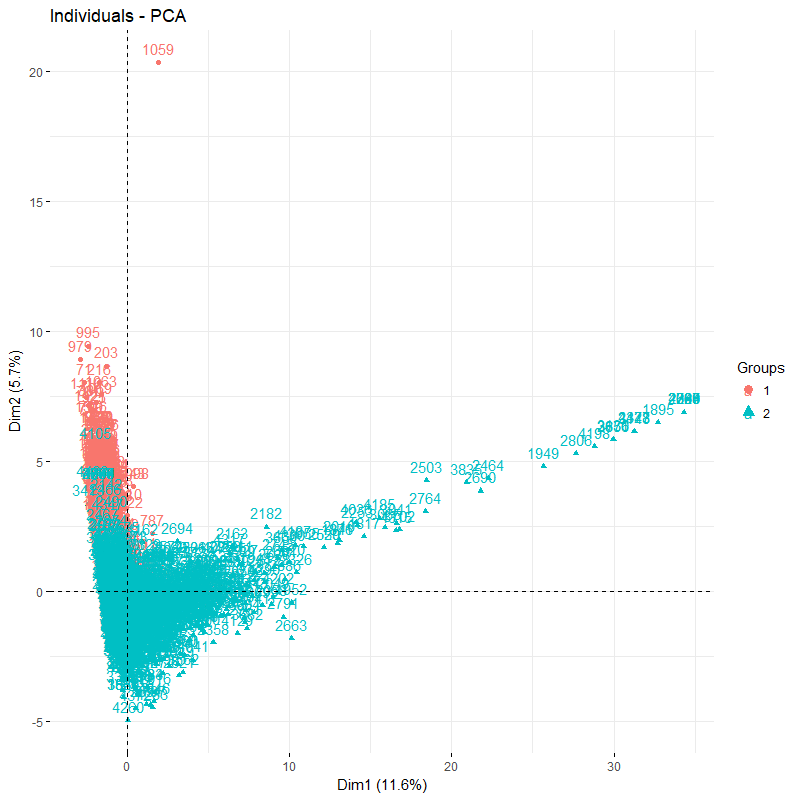
\includegraphics[scale = .3]{./discrimination/spambase/indi_plot12.png} &
    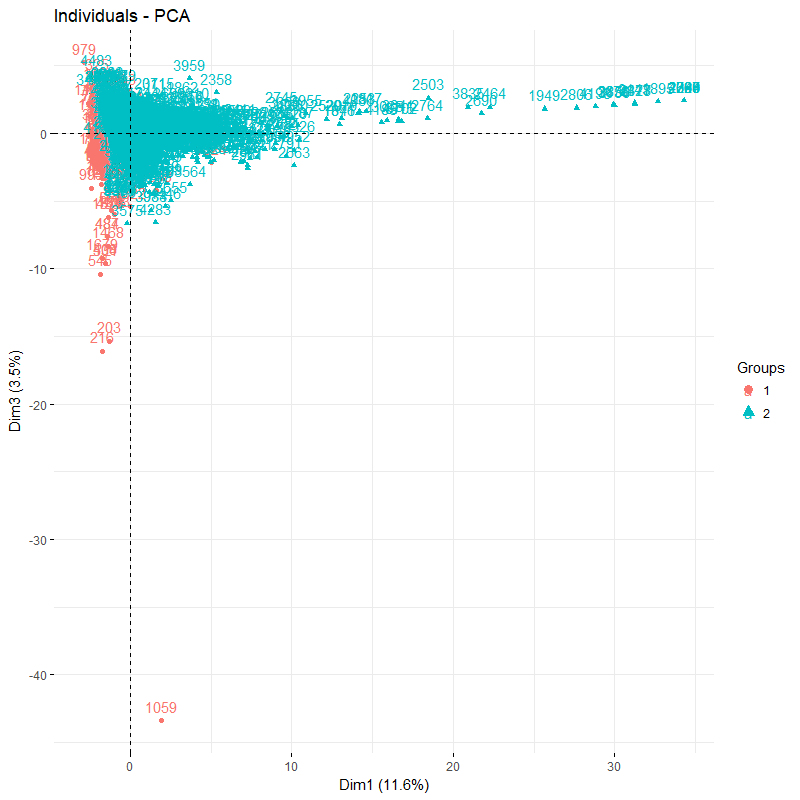
\includegraphics[scale = .3]{./discrimination/spambase/indi_plot13.png} 
    \end{tabular}
    \caption{La distribution des individus, graphique a : dans 2 premières composantes - graphique b : dans la 1me et 3ème composante \textbf{spambase}}
    \label{fig:my_label}
\end{figure}
\newline
La distribution des individus dans le graphique dans ce cas n'est pas claire. Nous avons visualisé des données dans les autres plans mais nous n'avons obtenu aucun meilleur résultat. Les deux classes ne sont pas séparées assez clairement pour une frontière linéaire donc nous pouvons prévoir que l'analyse de discriminante quadratique peut nous donner une classification plus précise. La régression logistique pourrais nous fournir une classification assez bonne car elle est assez flexible pour un jeu de données comme Spambase. Dans ce cas, la distribution des individus est compliquée pour que un modèle simple comme le classifieur bayésien naïf puisse nous donner un résultat agréable. L'arbre de décision peut performer assez bien dans ce cas parce que cette méthode est interprétable dans une grande dimension. Pour vérifier notre prédiction, nous viendrons la réalisation des méthodes de discrimination sur ce jeu de données.
\subsubsection{Réalisation des méthode de discrimination}
Pour calculer le taux d'erreur ponctuelle $\Hat{\epsilon}$ d'une prédiction, il faut simplement compter le nombre de prédiction erronées $\epsilon_i$ entre la prédiction faite et les données réelle (d'apprentissage ou de test), puis diviser par le nombre total d'individus \textit{n}. \newline
On répète cette procédure 100 fois pour obtenir 100 réalisations du taux d'erreur. Pour obtenir l'estimation du taux d'erreur $\Bar{\epsilon}$, il ne reste plus qu'à faire la moyenne des 100 réalisations. \newline
L'intervalle de confiance à 95\% est obtenu comme-ci : $IC = \left[\mu - 1.96*\frac{s^{*}}{\sqrt{N}};\mu + 1.96*\frac{s^{*}}{\sqrt{N}} \right]$ avec : \newline
\begin{itemize}
    \item $\mu$ : La moyenne des 100 réalisation de $\epsilon$ \\
    \item $s^{*}$ : L'écart-type corrigé des 100 réalisations de $\epsilon$ \\
    \item $N$ : Le nombre de réalisation et dans ce cas $N=100$
\end{itemize}
Nous avons d'abord essayé de réaliser les analyses avec le jeu de données initial. Les analyses discriminantes quadratique et linéaire et le classifieur bayésien naïf ne se fonctionnent pas et nous donne toujours des mêmes erreurs. Notre fonction de la régression logistique est bloquée car la dimension de ce jeu de données est très grande. Nous avons essayé des données pré-traitées mais rien ne marche. L'abre de décision est un seul modèle qui se fonctionne bien et donne un bon résultat car comme nous avons indiqué dessus, l'arbre de décision est interprétable même si dans la grande dimension. Nous ensuite cherchons à résoudre les problèmes avec l'analyse discriminante quadratique et linéaire, le classifieur bayésien naïf et avec la régression logistique. D'abord pour la régression logistique, on croit que le problème est la grande dimension du jeu de données et notre fonction doit réaliser trop de calculs, donc la vitesse est ralentie. C'est pourquoi elle ne peut pas retourner le résultat. Nous décidons d'utiliser une fonction \textit{glm} du bibliothèque \textbf{ISLR} pour augmenter la vitesse et performance de notre analyse. Pour le problème de l'analyse discriminante quadratique et linéaire et le classifieur bayésien naïf, nous avons d'abord cherché la raison qui produit des erreurs. Nous avons exploré le résultat retourné par la fonction \textbf{ad.val} que nous avons implémenté dans TD et nous avons trouvé quelques valeurs \textit{NaN} dans l'ensemble de probabilité et dans l'ensemble de classe prédite. Nous pouvons conclure ici que la risque $f_k = 0$ que nous avons prédite dans la partie d'analyse exploratoire se réalise. Le nombre de valeurs \textit{NaN} apparaissant dans le resultat rétourné par notre fonction dépend de la séparation de données en ensemble d'appentissage et de test mais il n'est jamais trop grand, maximum 5 valeurs \textit{NaN} sur 3068 individus dans l'ensemble d'apprentissage et sur 1533 individus dans l'ensemble de test. Donc on peut négligér ces valeurs \textit{NaN} car son effet n'est pas significatif. Nous avons modifié un peu notre code et toutes les analyses maintenant se fonctionne bien. De plus, comme nous avons discuté dans la partie d'analyse exploratoire, il y a quelques variables dont les valeurs sont beaucoup plus dominantes que les autres. Nous avons donc réalisé un pré-traitement sur ce jeu de données pour obtenir les résultats plus agréable que possible : nous dévisons chaque variable par sa valeur maximale et notre jeu de données devient des valeurs comprises entre 0 et 1. Nous réalisons l'ACP sur le jeu de données pré-traité et nous avons le graphique de individus ci-dessous. Nous pouvons voir que le jeu de données après le pré-traitement est plus visible, les individus sont plus séparés et se distribuent selon 2 groupes de variables.\newline
\begin{figure}[htb]
    \centering
    \begin{tabular}{ccc}
    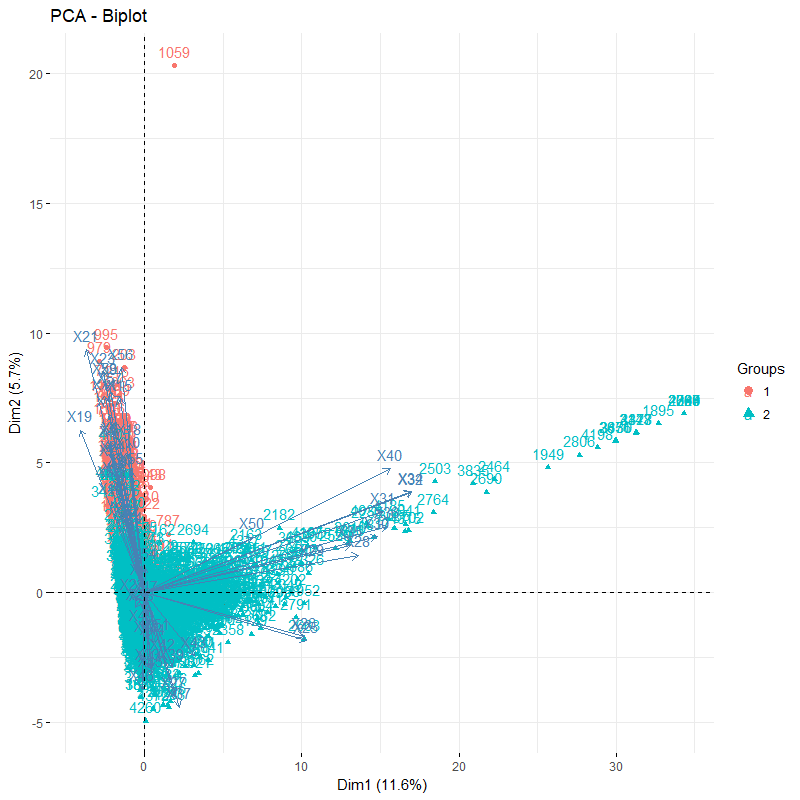
\includegraphics[scale = .3]{./discrimination/spambase/biplot4.png} &
    \end{tabular}
    \caption{La distribution des individus de \textbf{Spambase} après pré-traitement dans le premier plan}
    \label{fig:my_label}
\end{figure}
Nous avons puis appliqué des différents modèles d'analyses discriminantes, de régression logistique ainsi que les arbres de décisions. Le résume des résultats sont en table ci-dessous.
\begin{table}[H]
\centering

\begin{tabular}{l|l|cc}
\multicolumn{1}{l|}{\textbf{Méthode}}    & \textbf{Données} &$ \overline{\varepsilon}$ & $IC$                      \\ \hline
\multirow{2}{*}{Analyse discriminante quadratique} & Apprentissage    & 0.1588                   & $\left[0.1559 ;~ 0.1617 \right]$  \\
                                       & Test             &  0.1236             & $\left[0.1106  ;~ 0.1366 \right]$ \\ \hline
\multirow{2}{*}{Analyse discriminante linéaire}                  & Apprentissage & 0.1439                                 & $\left[0.1423 ;~ 0.1455 \right]$  \\
                                       & Test             & 0.1412                       & $\left[0.1384  ;~0.1441 \right]$ \\ \hline
\multirow{2}{*}{Classifieur bayésien naïf}                  & Apprentissage    &  0.1305                             & $\left[0.1272 ;~ 0.1338 \right]$  \\
                                       & Test             & 0.1311                                 & $\left[0.1280 ;~ 0.1342 \right]$ \\ \hline
\multirow{2}{*}{Régression logistique }                  & Apprentissage    &  0.0673                             & $\left[0.0655 ;~ 0.0691 \right]$  \\
                                       & Test             & 0.0743                                 & $\left[0.0719;~ 0.0768 \right]$ \\ \hline
\multirow{2}{*}{Arbre de décision}                  & Apprentissage    &  0.0972                             & $\left[0.0958 ;~  0.0987 \right]$  \\
                                       & Test             & 0.1071                                & $\left[0.1038 ;~ 0.1104 \right]$ 
\end{tabular}

\caption{Calcul du taux d'erreur d'apprentissage $\varepsilon$ et de test pour le jeu de données spambase avec plusieurs méthodes (arrondi à $10^{-4})$}
\label{spambase}
\end{table}
\begin{figure}[htb]
    \centering
    \begin{tabular}{cc}
    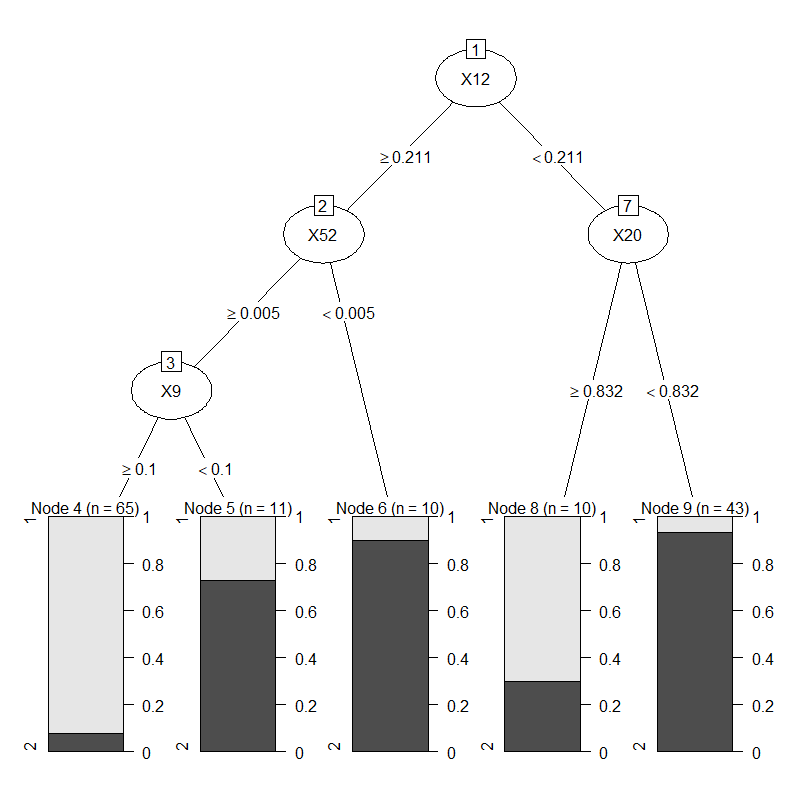
\includegraphics[scale = .4]{./discrimination/Sonar/tree_plot.png} &
    \end{tabular}
    \caption{L'arbre de décision \textbf{Sonar}}
    \label{fig:my_label}
\end{figure}
On remarque ici que dans le cas de la régression logistique quadratique, on ne peut pas réaliser l'analyse sur le jeu de données car dans certains cas nous obtenons ce résultat : $det(X^{T}W_{q}X) =  0$ donc il n'est pas possible d'inverser cette matrice.  
\newline
D'après la table \ref{spambase}, la régression logistique nous donne les meilleurs résultats. Comme ce que nous avons analysé dans la partie de l'ACP, les individus ne sont pas séparés très clairement (il y a beaucoup individus d'un groupe se situent dans un autre groupe) donc nous avons besoin d'un modèle assez flexible pour bien classifier les individus. Le classifieur bayésien naïf nous donne les taux d'erreurs assez forts car ce modèle est trop simple pour expimer ce jeu de données. L'analyse discriminante linéaire nous donne des taux assez grands et un peu plus que le classifieur bayésien naïf. On remarque ici que le jeu de données Spambase est complexe mais le classifieur bayésien naïf nous donne le meilleur resultat que l'analyse discriminante linéaire. L'analyse discriminante quadratique est une méthode aussi flexible mais dans ce cas elle nous donne un résultat qui n'est pas agréable parce que l'analyse discriminante quadratique doit estimer beaucoup de paramétres (dans ce cas le nombre de paramètres est de 3421 !). L'arbre de décision nous donne toujours un bon résultat. \newline


\subsection{Spambase 2}
\subsubsection{Analyse exploratoire}
Comme le jeu de données précédent, nous avons d'abord effectué une analyse exploratoire pour comprendre et s'approcher les données fournies. \newline
Ce jeu de données comporte 57 variables et 4601 individus comme le jeu de données précédent. On a exclu la première colonne parce que cela correspond à l'index qui est inutile dans notre analyse.
\begin{figure}[htb]
    \centering
    \begin{tabular}{cc}
    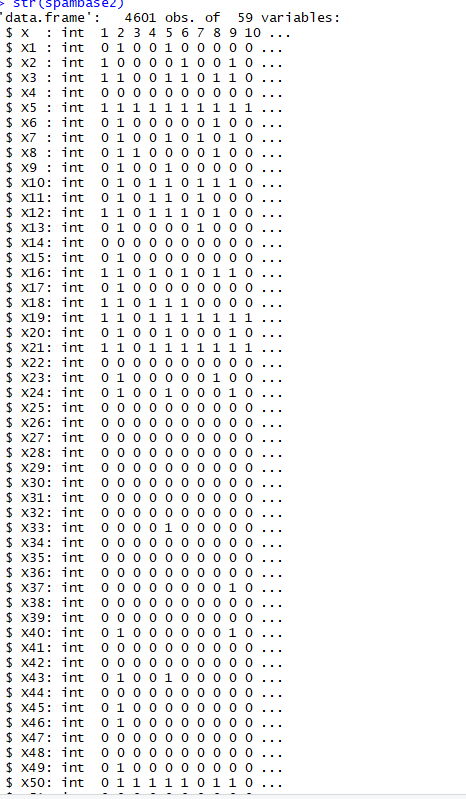
\includegraphics[scale = .3]{./discrimination/spambase2/str.PNG} &
    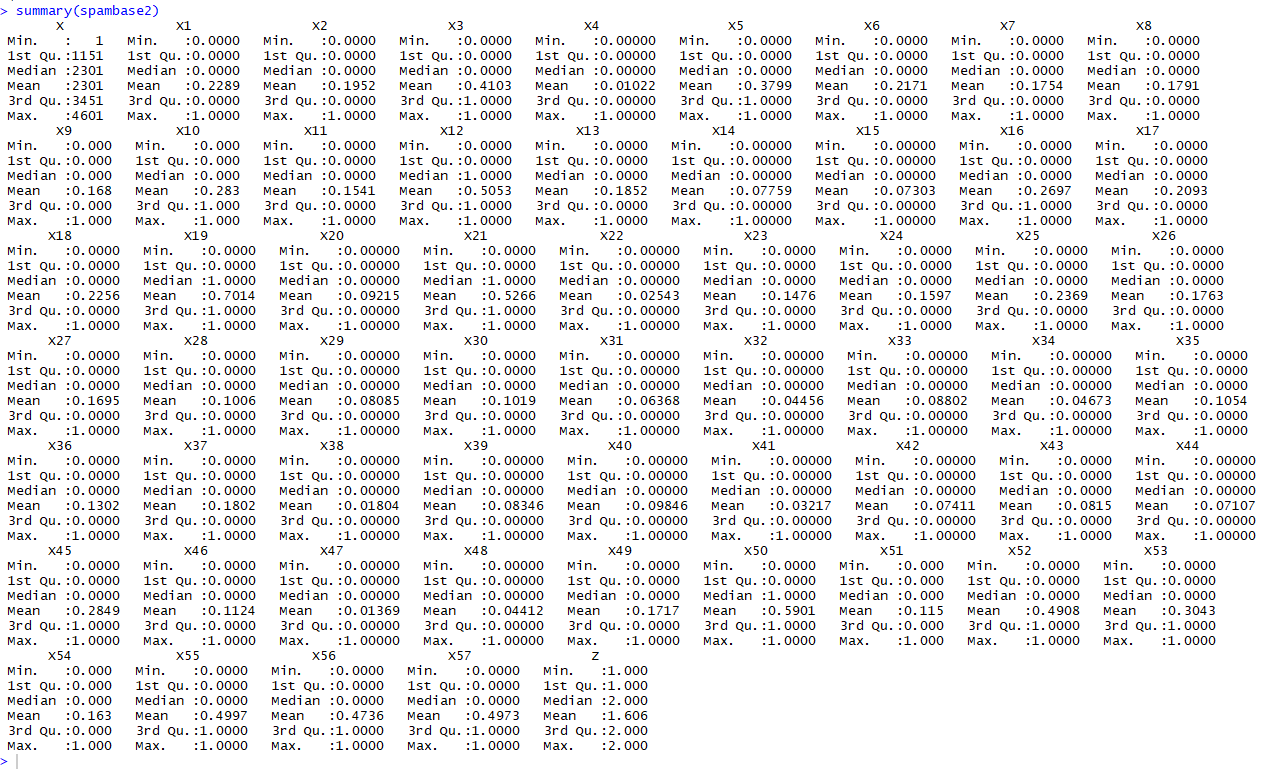
\includegraphics[scale = .3]{./discrimination/spambase2/summary.PNG}
    \end{tabular}
    \caption{La strucutre du jeu de données \textbf{spambase2}}
    \label{fig:my_label}
\end{figure}
A partir des résultats ci-dessus, on peut voir que toutes les variables sont des variables binaire. On puis étudie la corrélation des variables.
\newline
\begin{figure}[htb]
    \centering
    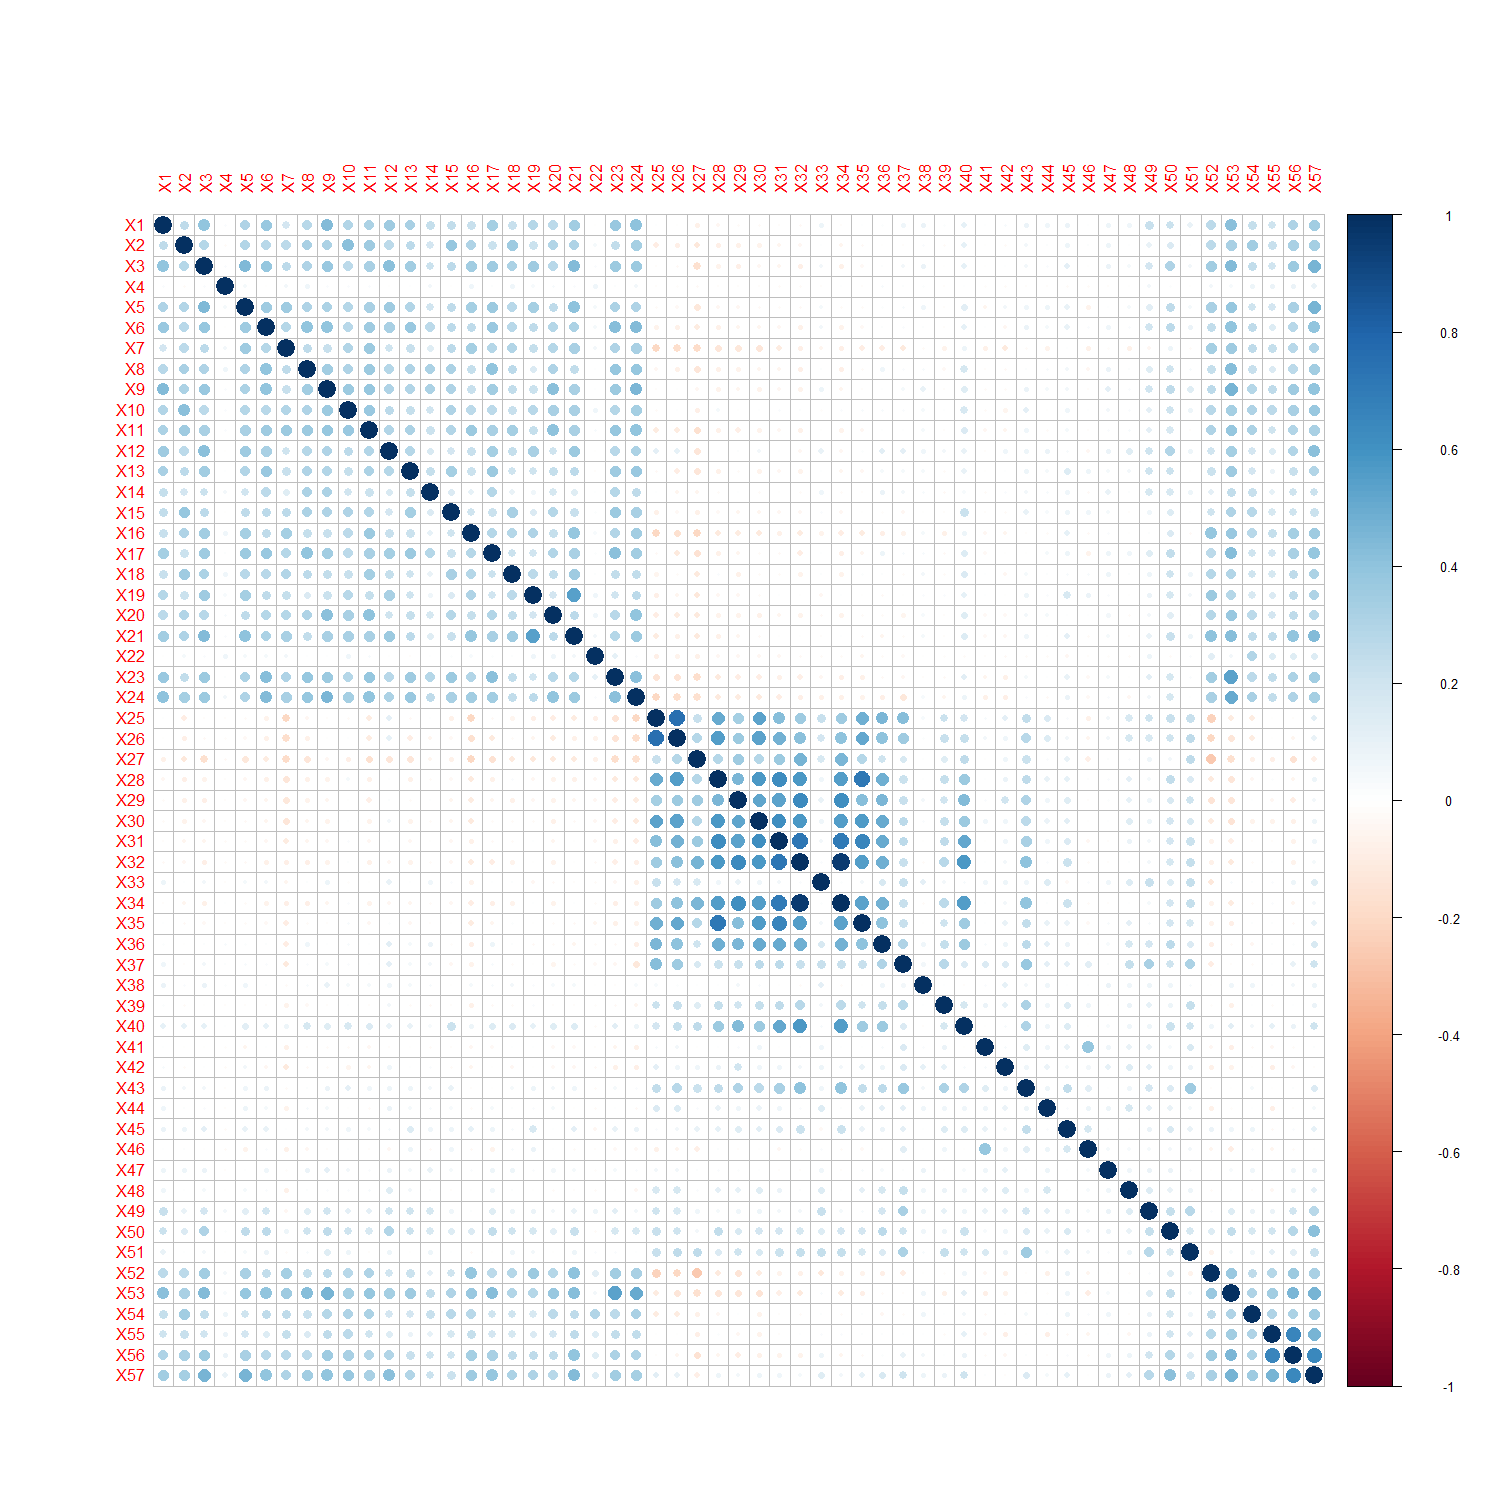
\includegraphics[scale = .2]{./discrimination/spambase2/corrplot.png} 
    \caption{La corrélation entre les variables de \textbf{spambase2}}
    \label{my_label}
\end{figure}
Le test de corrélations a été réalisé par la méthode de Pearson avec \textbf{p-value} a été fixée par défault pour $\alpha = 0.05$. Grâce au graphique, on peut observer la corrélation entre des variables n'est pas significative sauf le couple $(X34,X36)$. Comme l'étude précédent, on veut au premier temps explorer la géométrie des données et à partir de cela, on peut prévoir le modèle compatible. \newline
Nous avons obtenu d'abord 2 graphiques : le cercle de corrélation et l'inertie de valeurs propres de 10 premières valeurs en utilisant la fonction \textit{princomp} et des fonctions du biliothèque \textit{factoextra}.
\begin{figure}[htb]
    \centering
    \begin{tabular}{c|c}
    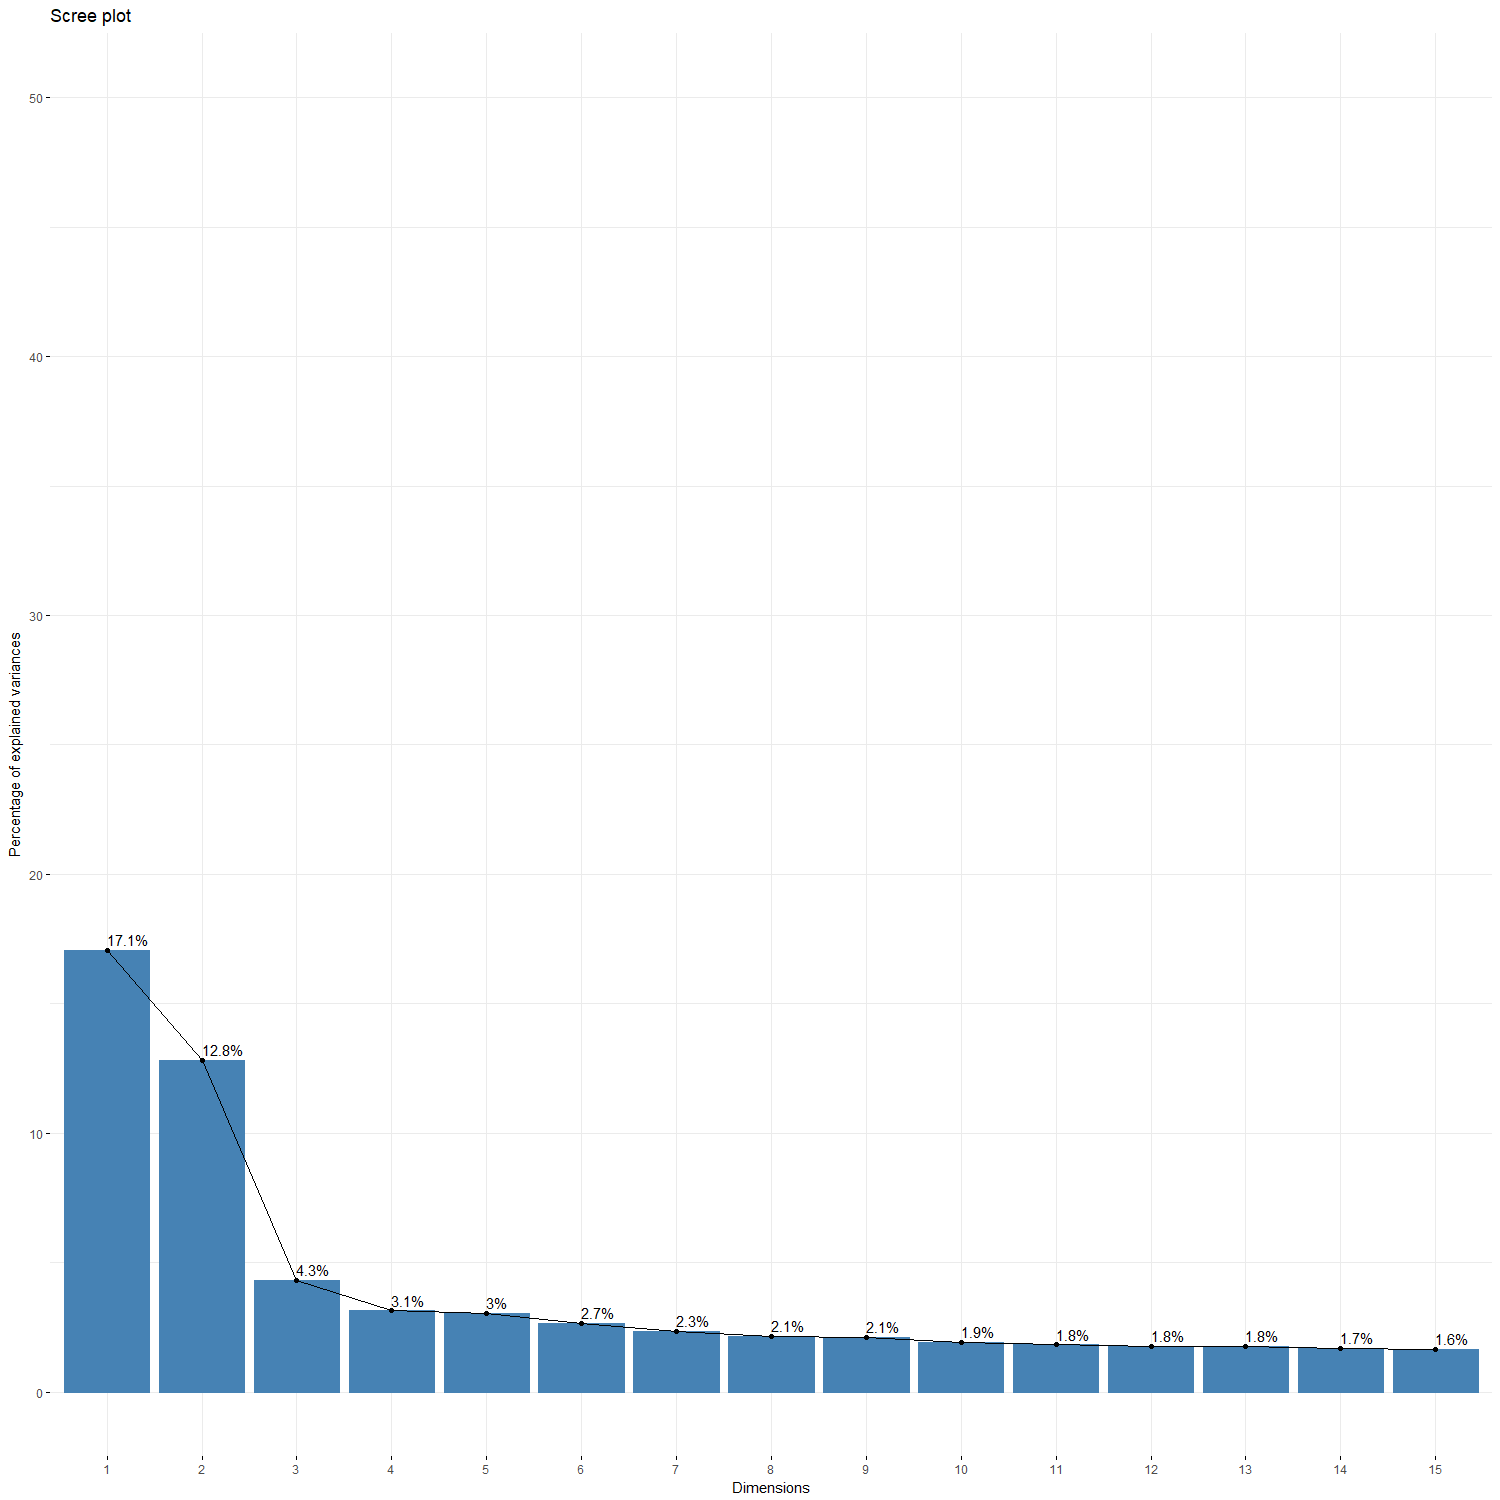
\includegraphics[scale = .1]{./discrimination/spambase2/eig_plot.png} &
    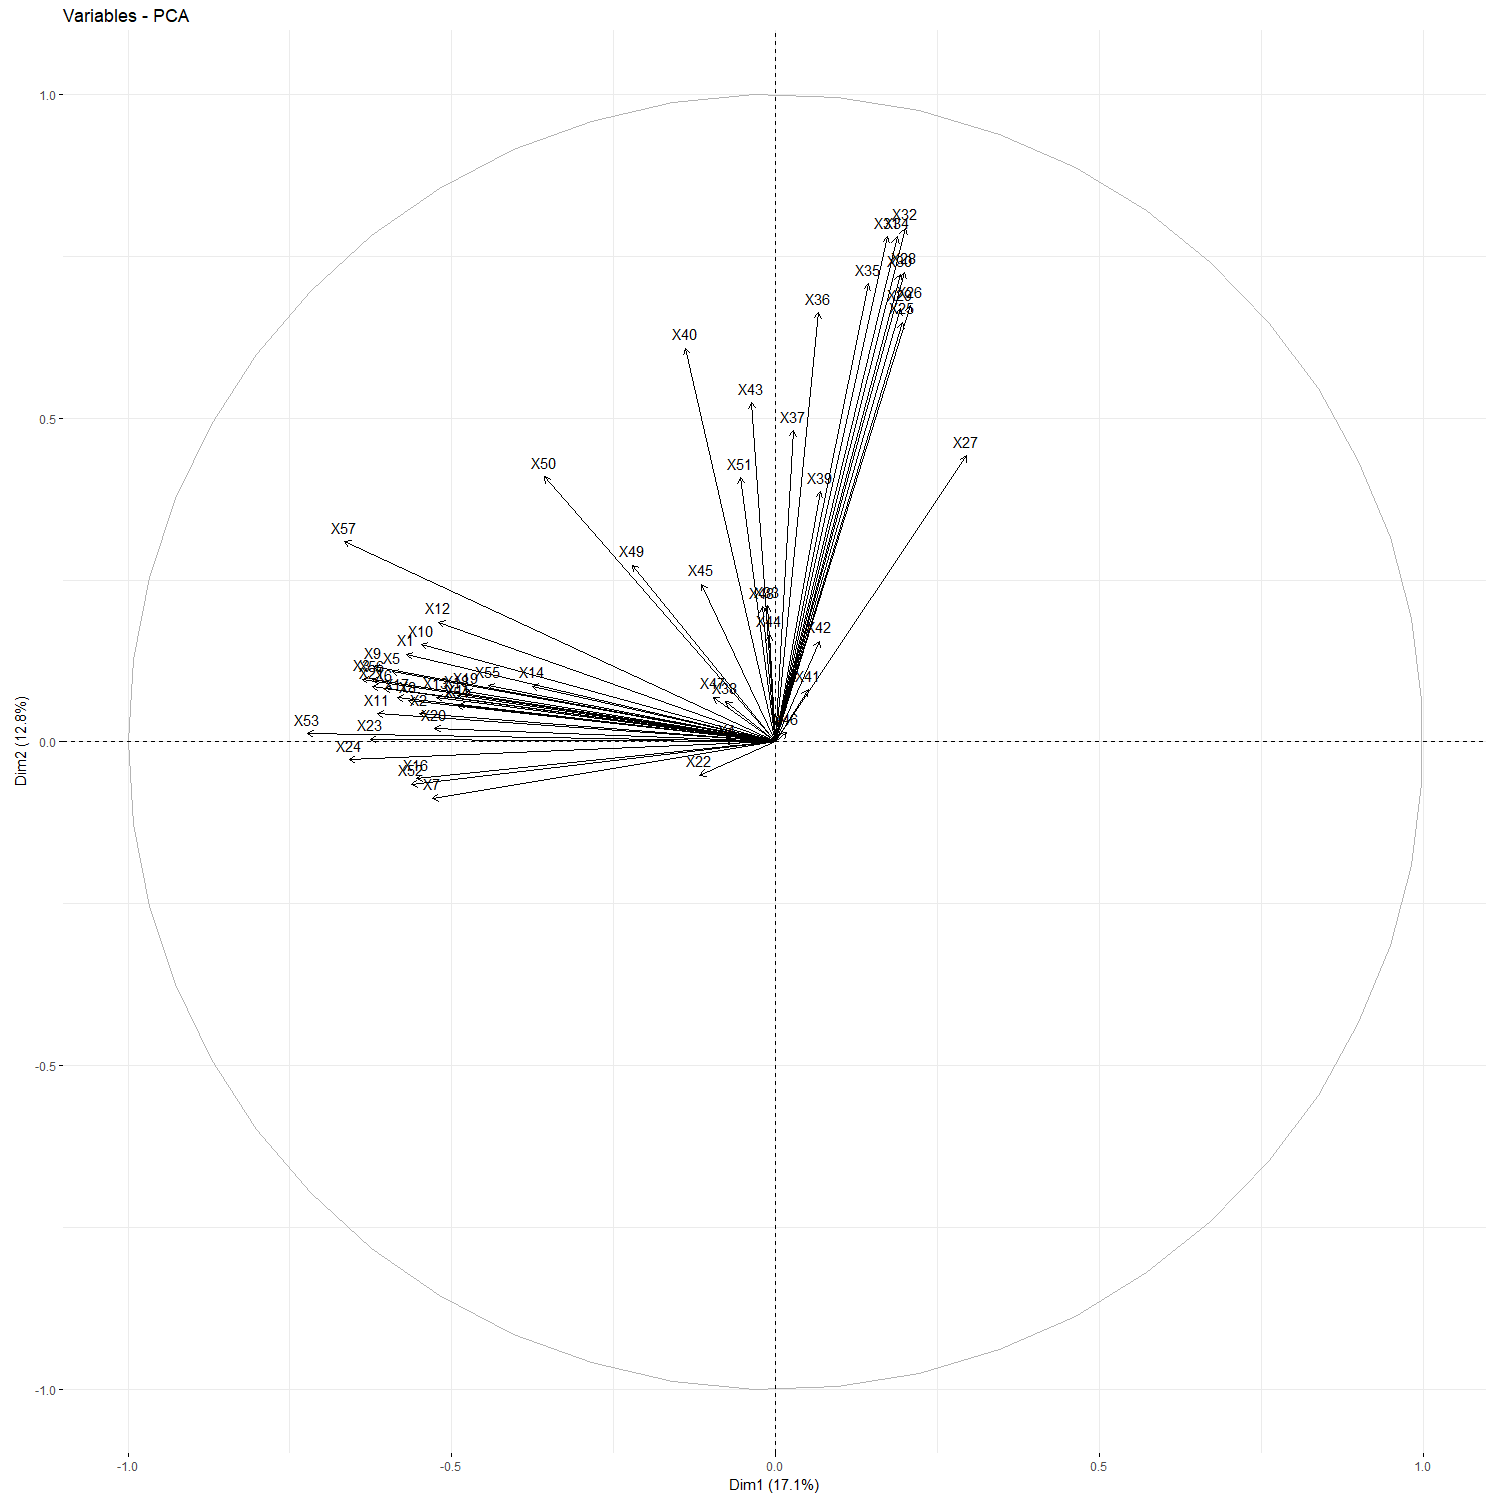
\includegraphics[scale = .1]{discrimination/spambase2/varplot.png}
\end{tabular}
    \caption{Graphique a : L'inertie de valeurs propres de 10 premières valeurs - Graphique b : Le cercle de corrélation des variables \textbf{Sonar}}
    \label{fig:my_label}
\end{figure}
Dans le cadre de notre analyse, nous pouvons voir que les informations se concentrent aux 45 premières composantes avec plus de 92\% des informations totales. De plus, le cercle de corrélation des variables expliqué par les deux premières composantes nous montre la corrélation entre les variables. Nous pouvons vois que les variables groupent en 2 groupes principaux : un groupe selon la première composante et un autre selon la deuxième composante. On observe la distribution des individus dans le graphique des individus ci-dessous. 
\begin{figure}[htb]
    \centering
    \begin{tabular}{ccc}
    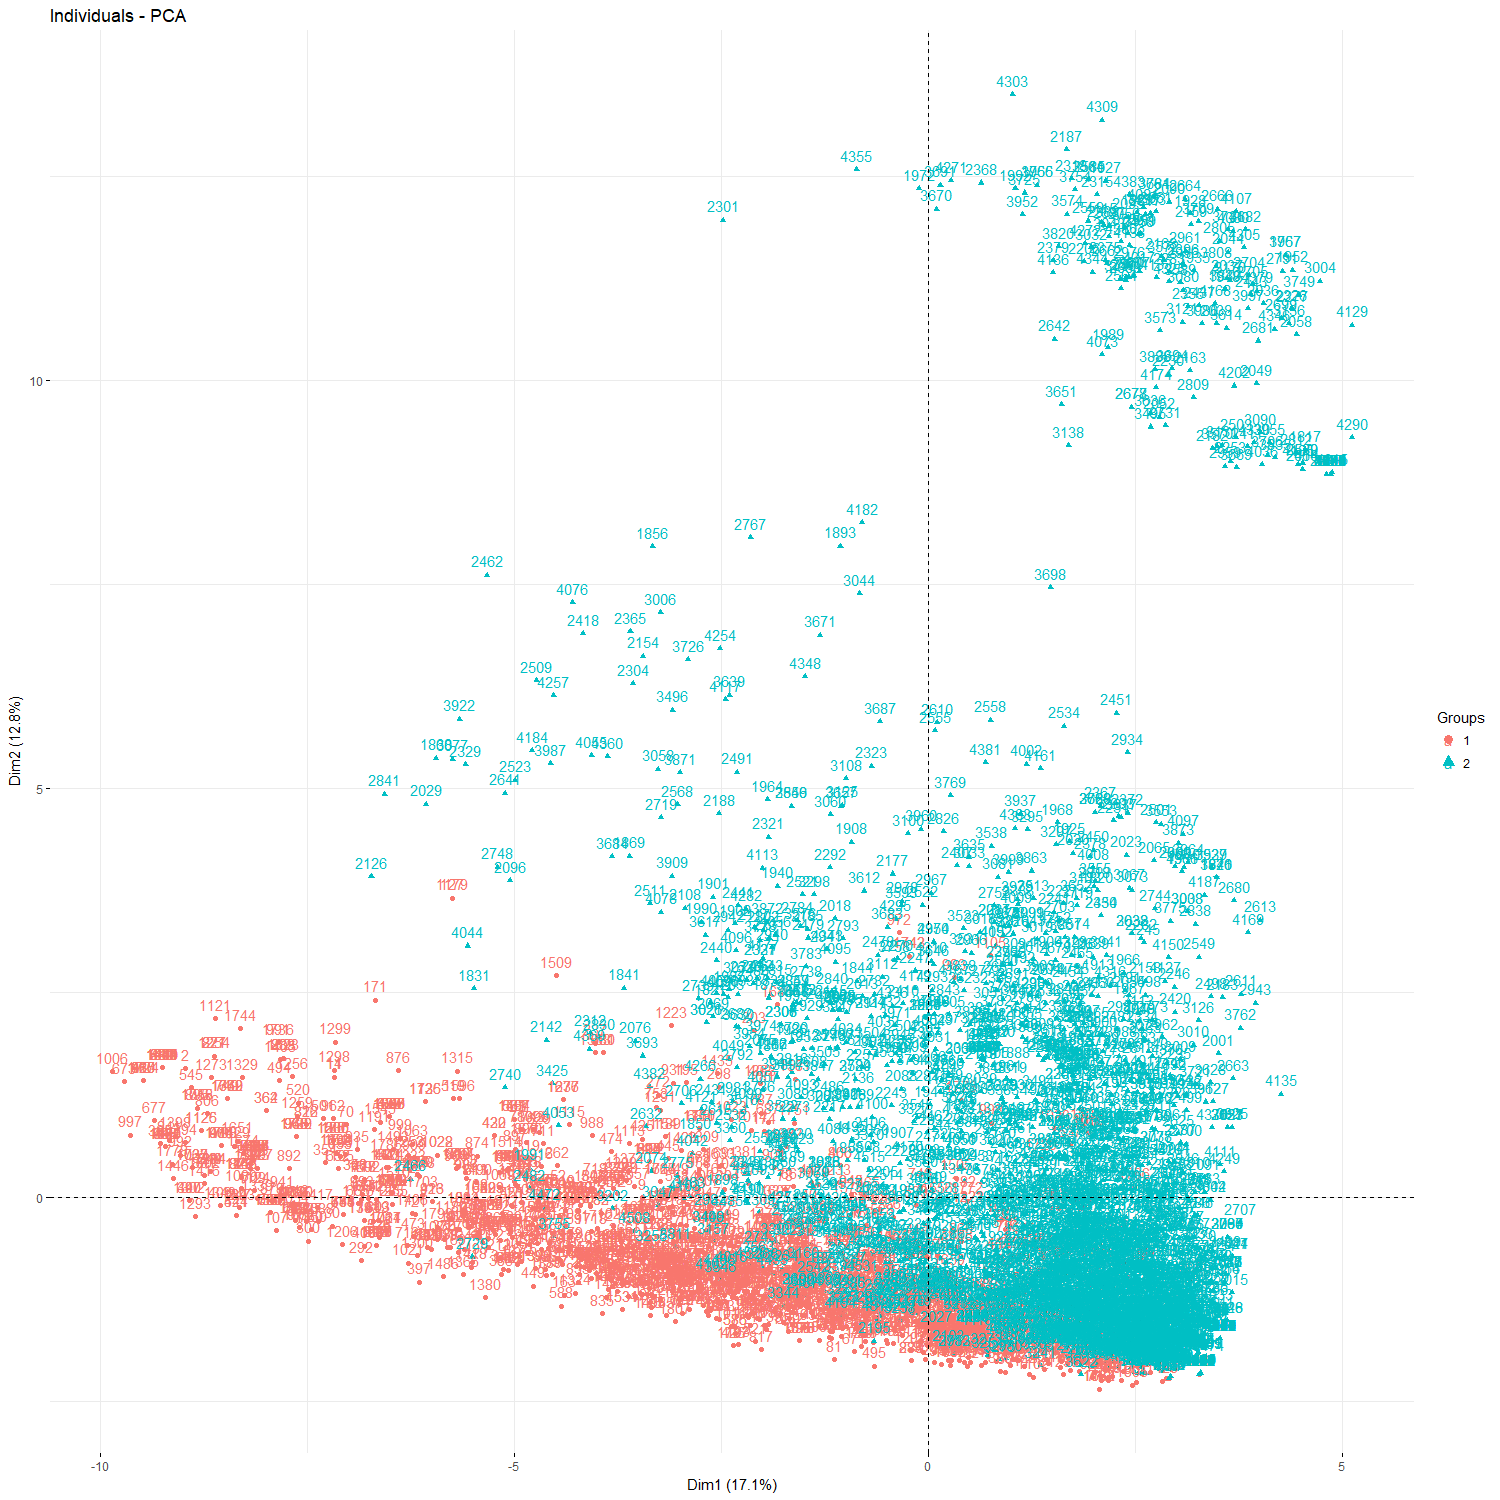
\includegraphics[scale = .1]{./discrimination/spambase2/indi_plot12.png} &
    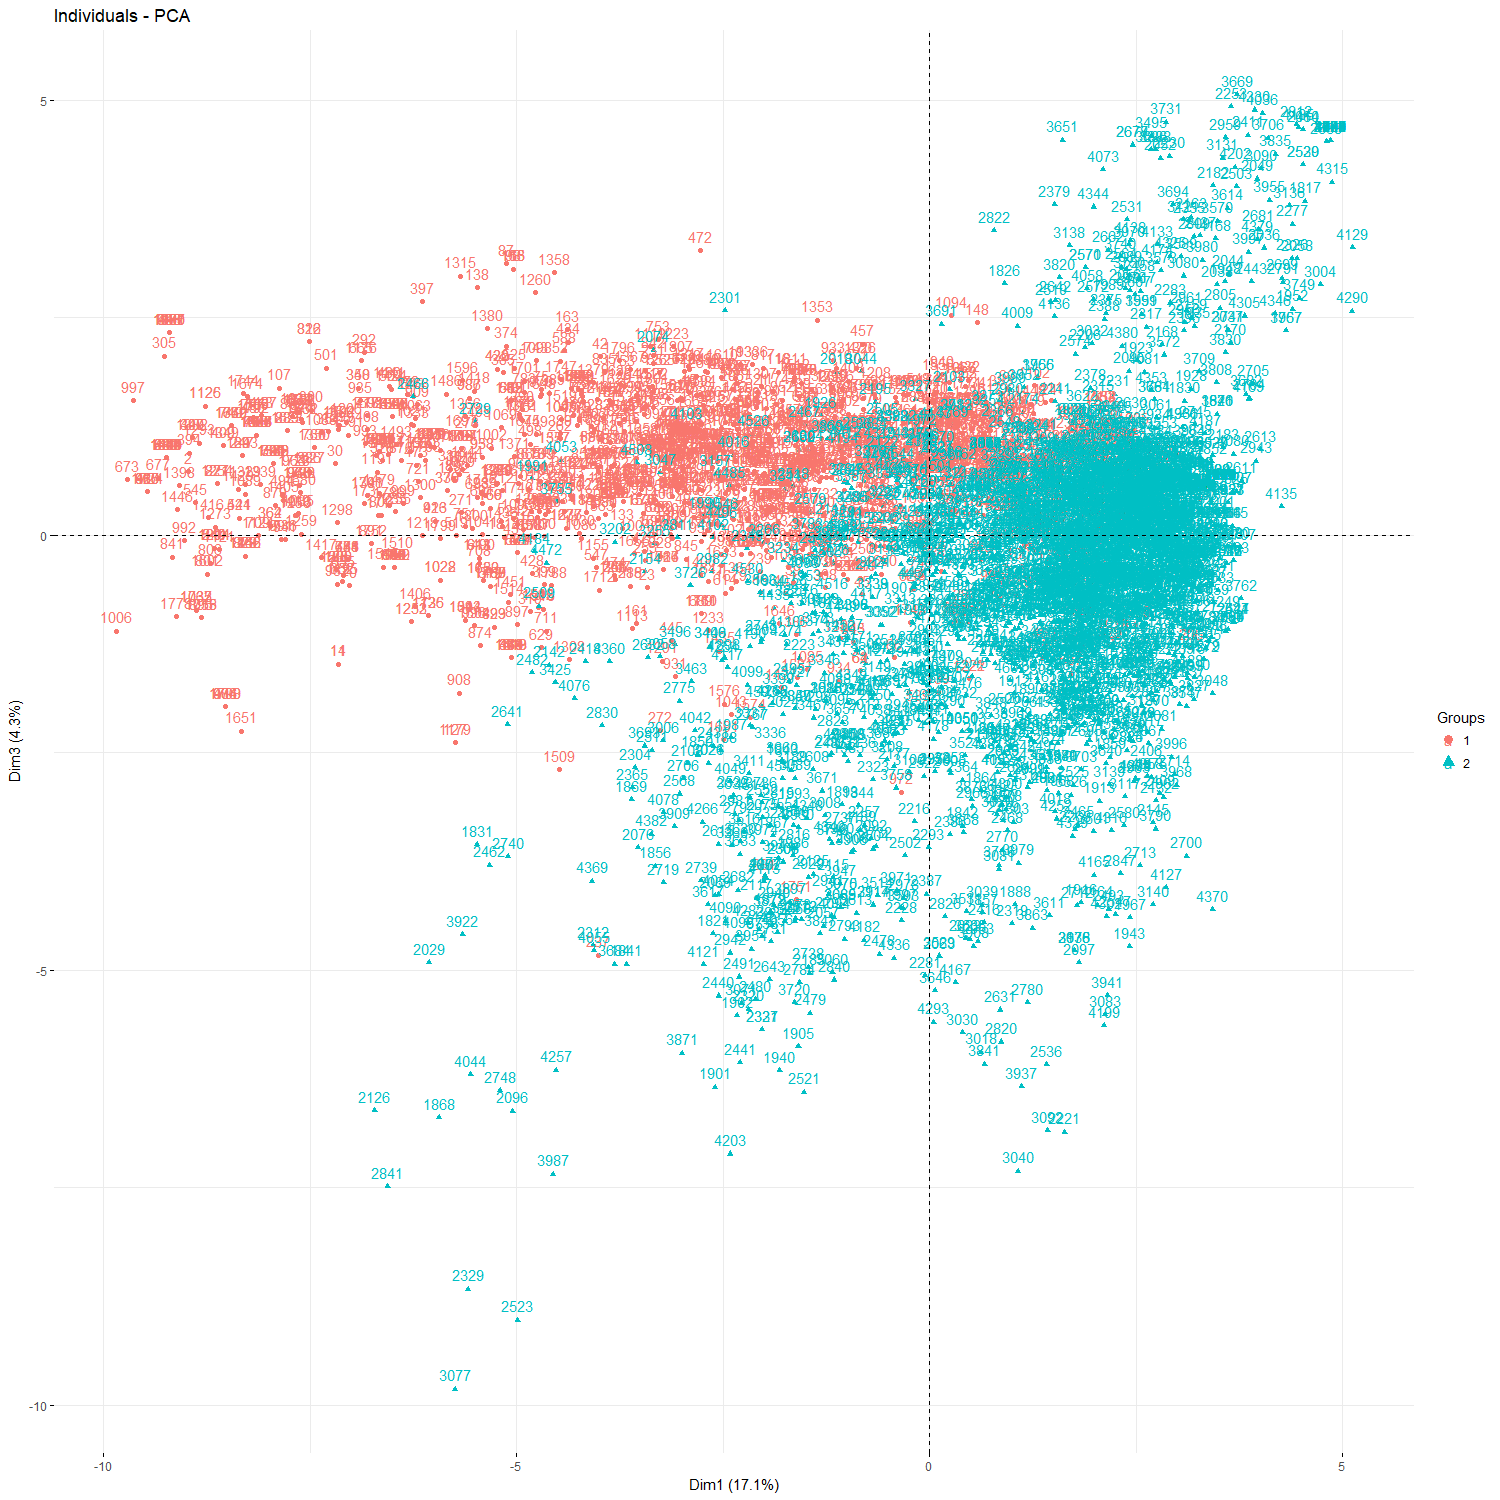
\includegraphics[scale = .1]{./discrimination/spambase2/indi_plot13.png} 
    \end{tabular}
    \caption{La distribution des individus, graphique a : dans 2 premières composantes - graphique b : dans la 1me et 3ème composante \textbf{spambase2}}
    \label{fig:my_label}
\end{figure}
\newline
La distribution des individus dans le graphique dans ce cas n'est plus très claire. Nous pouvons voir que dans la $1^{ère}$ et $3^{ème}$ composante principale, les individus de groupe 1 ont tendance de se situer selon le groupe de variables qui est se distribuent selon la première composante tandis que les individus de groupe 2 ont tendance de se concentrer au centre. Avec ce jeu de données peu d'individus comme \textbf{Spambase 2}, le modèle flexible peut nous donner des resultats agréables comme l'analyse discriminante quadratique ou la régression logistique mais l'analyse discriminante quadratique nous donnerais un taux d'erreurs plus significatifs que la régression logistique car il y a beaucoup de paramètres à estimer. De plus, l'arbre de décision peut bien fonctionner dans un jeu de données à grande dimension comme \textbf{Spambase 2}. Pour vérifier notre prédiction, nous viendrons la réalisation des méthodes de discrimination sur ce jeu de données. 
\subsubsection{Réalisation des méthode de discrimination}
Pour calculer le taux d'erreur ponctuelle $\Hat{\epsilon}$ d'une prédiction, il faut simplement compter le nombre de prédiction erronées $\epsilon_i$ entre la prédiction faite et les données réelle (d'apprentissage ou de test), puis diviser par le nombre total d'individus \textit{n}. \newline
On répète cette procédure 100 fois pour obtenir 100 réalisations du taux d'erreur. Pour obtenir l'estimation du taux d'erreur $\Bar{\epsilon}$, il ne reste plus qu'à faire la moyenne des 100 réalisations. \newline
L'intervalle de confiance à 95\% est obtenu comme-ci : $IC = \left[\mu - 1.96*\frac{s^{*}}{\sqrt{N}};\mu + 1.96*\frac{s^{*}}{\sqrt{N}} \right]$ avec : \newline
\begin{itemize}
    \item $\mu$ : La moyenne des 100 réalisation de $\epsilon$ \\
    \item $s^{*}$ : L'écart-type corrigé des 100 réalisations de $\epsilon$ \\
    \item $N$ : Le nombre de réalisation et dans ce cas $N=100$
\end{itemize}
Nous avons puis appliqué des différents modèles d'analyses discriminantes, de régression logistique ainsi que les arbres de décisions. Le résume des résultats sont en table ci-dessous.
\begin{table}[H]
\centering

\begin{tabular}{l|l|cc}
\multicolumn{1}{l|}{\textbf{Méthode}}    & \textbf{Données} &$ \overline{\varepsilon}$ & $IC$                      \\ \hline
\multirow{2}{*}{Analyse discriminante quadratique} & Apprentissage    & 0.0680                   & $\left[0.0674 ;~ 0.0686 \right]$  \\
                                       & Test             & 0.0762            & $\left[0.0750  ;~ 0.0773 \right]$ \\ \hline
\multirow{2}{*}{Analyse discriminante linéaire}                  & Apprentissage & 0.1057                                 & $\left[0.1050 ;~ 0.1063 \right]$  \\
                                       & Test             & 0.1094                      & $\left[0.1079  ;~0.1108 \right]$ \\ \hline
\multirow{2}{*}{Classifieur bayésien naïf}                  & Apprentissage    &  0.1695                            & $\left[0.1680 ;~ 0.1709 \right]$  \\
                                       & Test             & 0.1669                                 & $\left[0.1629 ;~0.1709 \right]$ \\ \hline
\multirow{2}{*}{Régression logistique }                  & Apprentissage    &  0.0559                             & $\left[ 0.0548 ;~ 0.0570 \right]$  \\
                                       & Test             & 0.0621                                 & $\left[0.0597;~ 0.0644 \right]$ \\ \hline
\multirow{2}{*}{Arbre de décision}                  & Apprentissage    &  0.1126                             & $\left[0.1113 ;~ 0.1139 \right]$  \\
                                       & Test             &  0.1190                                 & $\left[0.1174 ;~ 0.1207 \right]$ 
\end{tabular}

\caption{Calcul du taux d'erreur d'apprentissage $\varepsilon$ et de test pour le jeu de données spambase 2 avec plusieurs méthodes (arrondi à $10^{-4})$}
\label{spambase2}
\end{table}
\begin{figure}[htb]
    \centering
    \begin{tabular}{cc}
    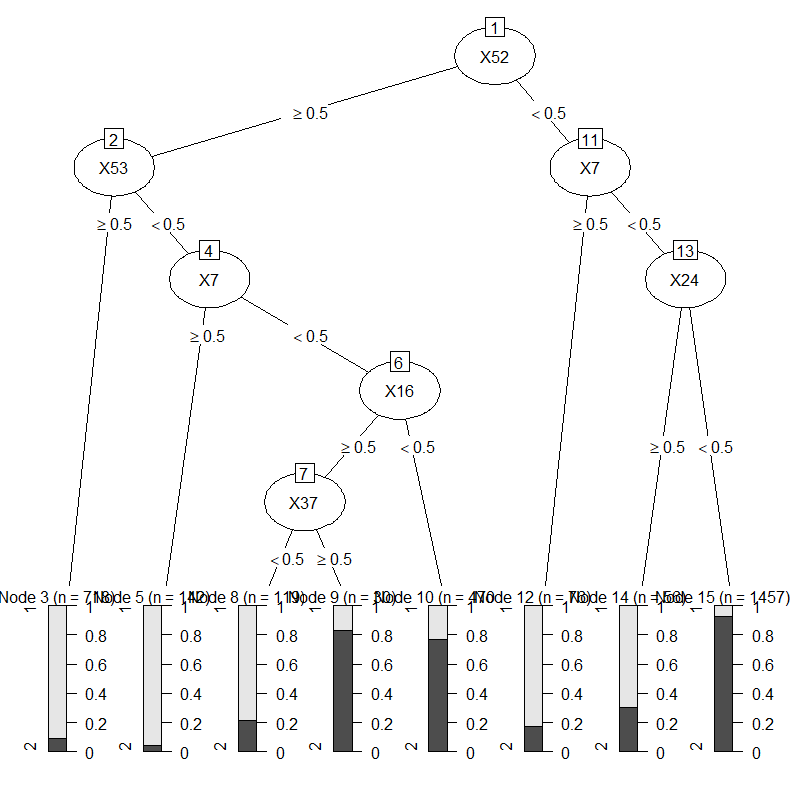
\includegraphics[scale = .4]{./discrimination/spambase2/treeplot.png} &
    \end{tabular}
    \caption{L'arbre de décision \textbf{Spamebase 2}}
    \label{fig:my_label}
\end{figure}
On remarque ici que dans le cas de la régression logistique, on ne peut pas réaliser l'analyse sur le jeu de données par notre fonction le jeu de données comporte trop de variables et observations donc notre fonction doit réaliser beaucoup de calculs. C'est pourquoi la vitesse est ralentie et elle ne peut pas retourner le resultat. Donc nous avons utilisé la fonction \textit{glm} du bibliothèque \textbf{ISLR}. 
\newline
D'après la table \ref{spambase2}, la régression logistique nous donne les meilleurs résultats. Comme ce que nous avons analysé dans la partie de l'ACP, les individus ne sont pas séparés très clairement (il y a beaucoup individus d'un groupe se situent dans un autre groupe) donc nous avons besoin d'un modèle assez flexible pour bien classifier les individus. L'analyse discriminante quadratique nous donne également un très bon resultat. L'analyse discriminante quadratique et la régression logistique sont assez complexe pour exprimer des données. Le classifieur bayésien naïf nous donne les taux d'erreurs assez forts car ce modèle est trop simple pour expimer ce jeu de données. L'analyse discriminante linéaire peut nous donner un resultat acceptable car ce modèle est plus robuste que le classifieur bayésien naïf mais il n'est pas assez flexible pour ce jeu de données. Malgré à la grande dimension, l'arbre de décision nous donne aussi un resultat stable.  


\end{document}

